% !TEX TS-program = xelatex
\documentclass[profonts,stix,handout]{astro-bookshelf}
\hypersetup{colorlinks=true,linkcolor=blue,citecolor=black,urlcolor=blue}

\usepackage{aasjournals}
\usepackage{wasysym}

\graphicspath{{frontmatter/}{coordinates/figs/}{light-telescopes/figs/}{detection-exoplanets/figs/}{beyond-kepler/figs/}{resonance/figs/}{planetary-atmospheres/figs/}{constants-units/figs/}{math-review/figs/}{statistics/figs/}}

\usepackage[units,derivatives,vectors,code,symbols]{starType}
\newcommand*{\rhat}{\ensuremath{\bvec{\hat{r}}}}
\newcommand*{\thetahat}{\ensuremath{\bvec{\hat{\theta}}}}
\newcommand*{\rv}{\ensuremath{\bvec{r}}}
\newcommand*{\xv}{\ensuremath{\bvec{x}}}
\newcommand*{\DDtt}[1]{\frac{\dif^{2} #1}{\dif t^{2}}}

\newcommand*{\Earth}{\oplus}
\newcommand*{\Moon}{\leftmoon}

\newcommand*{\joule}{\unitstyle{J}}
\newcommand*{\watt}{\unitstyle{W}}

\newcommand*{\RA}{\ensuremath{\mathrm{RA}}}
\newcommand*{\dec}[3]{%
	\ifthenelse{\isempty{#3}}%
		{\ensuremath{#1^{\circ}\,#2'}}
		{\ensuremath{#1^{\circ}\,#2'\,#3''}}}
\newcommand*{\hrangle}[3]{%
	\ifthenelse{\isempty{#3}}%
		{\ensuremath{#1^{\mathrm{h}}\,#2^{\mathrm{m}}}}
		{\ensuremath{#1^{\mathrm{h}}\,#2^{\mathrm{m}}\,#3^{\mathrm{s}}}}}

\newcommand*{\prob}{\ensuremath{\mathcal{P}}}
\newcommand*{\mean}[1]{\ensuremath{\left\langle#1\right\rangle}}
\newcommand*{\binom}[3]{\ensuremath{\prob_{#1}(#2;#3)}}
\newcommand*{\expect}{\ensuremath{\mathcal{E}}}

\newcommand*{\wt}{\omega t}
\newcommand*{\wot}{\omega_{0} t}
\newcommand*{\wmt}{\omega_{m} t}
\newcommand*{\womw}{(\omega_{0}^{2}-\omega^{2})}
\newcommand*{\gw}{(\Gamma/m)^{2}\omega^{2}}


\newcommand*{\maintitle}{Planets and Telescopes}
\newcommand*{\notice}{\thanks{Excerpt from \maintitle, git version \input{git-info}\ldots. \ccCopy\ 2015 Edward Brown; \ccbyncsa\ Except where explicitly noted, this work is licensed under the Creative Commons
Attribution-NonCommercial-ShareAlike 4.0 International (CC BY-NC-SA
4.0) license.}}

\title{Coordinates: Specifying Locations on the Sky}
% \title{Light and Telescopes}
% \title{Detection of Exoplanets}
% \title{Beyond Kepler's Laws}
% \title{Resonances in the Solar System}
% \title{Planetary Atmospheres}
% \title{Constants and Units}
% \title{Mathematics Review}
% \title{Probability and Statistics}

\author{Edward Brown}
%\publisher{Open Astrophysics Bookshelf}
\date{6 June 2015}

\begin{document}
\maketitle

%!TEX root = ../AST208-notes.tex

\section{Declination and right ascension}
To talk about events in the sky, we need to specify where they are located. To specify where they are located, we need a point of reference.  This is a bit tricky: we are riding on the Earth, which rotates and orbits the Sun; the Sun orbits the Milky Way; the Milky Way moves through the Local Group; and on top of all this the universe is expanding.

The primary criterion for choosing a coordinate system is convenience. We want a system that is easy to use and that describes the sky straightforwardly.
As viewed from Earth, we appear to be at the center of a great sphere, with celestial objects lying on its surface. This is similar to describing locations on the Earth, for which we use two angles: latitude, which measures the angle north or south from the equator; and longitude, which measures the angle east or west from the prime meridian.  Likewise, to describe the apparent position of objects as viewed from Earth, we also need two angles.

\begin{marginfigure}
\includegraphics[width=\linewidth]{celestial-sphere}
\caption[The celestial sphere]{The meridian (red) passing through our zenith (Z).  Our vantage point is from the center of the sphere. Also shown are the north celestial pole (NCP), south celestial pole (SCP) and the celestial equator (CE).  The shaded region are points below our horizon; objects in that region are not visible from our location. A star with negative declination $\delta$ is shown as well.}
\label{f.meridian}
\end{marginfigure}

First, let's describe our measurement of position on the sky.
The local gravitational acceleration $\bvec{g}$ specifies the \emph{local vertical}; this picks out a point on the celestial sphere, our \emph{zenith}.  Our \emph{horizon} is then defined by points that lie $90^{\circ}$ from this zenith, measured along a great circle passing through the zenith.  The zeniths above the north and south poles define the \emph{north and south celestial poles}.  A great circle connecting the celestial poles and our zenith defines our \emph{meridian} (see Fig.~\ref{f.meridian}).  As the Earth rotates, celestial objects appear to move westward on circles about the celestial poles.  

Midway between the north and south celestial poles lies the celestial equator.  For any star, you specify its declination $\delta$ as the angle north (positive) or south (negative) of the celestial equator along that star's meridian.  For example, Betelgeuse, the red star in the shoulder of Orion, has a declination $\delta = \dec{7}{24}{25}$.  Polaris, the North star, has $\delta = \dec{89}{15}{51}$.
\marginnote[-2\baselineskip]{Declination is quoted in degrees ($^{\circ}$), arcminutes ($'$), and arcseconds ($''$).  There are 60 arcminutes in 1 degree and 60 arcseconds in 1 arcminute.}

\begin{exercisebox}[Altitude of Betelgeuse]
How far above our southern horizon will Betelgeuse be when it crosses our meridian? Our latitude is \dec{42}{43}{25}N.
\end{exercisebox}

Declination measures how far north or south of the celestial equator a given object lies. To specify an east-west location, we need another reference point.  Because of the Earth's rotation, we can't use a point on Earth, such as the Greenwich observatory (which is where the $0^{\circ}$ of longitude is defined).  We can, however, use the Earth's motion around the Sun: as the Earth moves around the Sun, the Sun appears to move eastwards relative to the fixed stars. This path the Sun takes around the celestial sphere is known as the \emph{ecliptic}, and the constellations that lie along the ecliptic are the \emph{zodiac}.
Because the Earth's rotational axis is tilted at an angle of \dec{23}{16}{} with respect to its orbital axis, the Sun's declination varies over the course of a year.   

\begin{figure}[hb]
\includegraphics[width=\linewidth]{ecliptic}
\caption[The ecliptic]{As Earth orbits the Sun, the Sun's declination traces out a path along the celestial sphere known as the \emph{ecliptic}.  Over the course of a year, the Sun appears to move eastward, relative to distant stars, along the ecliptic.}
\label{f.ecliptic}
\end{figure}

The Sun reaches its minimum declination, \dec{-23}{16}{}, when it appears to lie in the direction of Sagittarius at the \emph{winter solstice}.  One quarter orbit later, the Sun crosses the celestial equator; at this point the Sun is in the direction of Pisces at the \emph{vernal equinox}. Another quarter orbit brings the Sun in the direction of Gemini with declination \dec{23}{16}{}; this is the \emph{summer solstice}. A further quarter orbit, and the Sun crosses the celestial equator in the direction of Virgo at the \emph{autumnal equinox}.

The ecliptic thus intersects the celestial equator at two points (Fig.~\ref{f.ecliptic}), the \emph{vernal and autumnal equinoxes}. We usually associate the equinoxes with a specific time of year, but they actually define unique directions on the sky. We can therefore define our second angular coordinate, \emph{right ascension}, as the angle between an objects' meridian and the vernal equinox, measured eastwards along the celestial equator.

\begin{marginfigure}
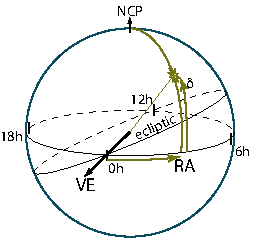
\includegraphics[width=\linewidth]{right-ascension}
\caption[Right ascension and declination]{The right ascension (\RA) and declination ($\delta$) of a celestial object.}
\label{f.right-ascension}
\end{marginfigure}

Rather than specify the right ascension by degrees, astronomers instead quote it in terms of hours (and minutes and seconds).  The vernal equinox is therefore at $\RA = \hrangle{00}{00}{00}$ and the autumnal equinox is at $\RA = \hrangle{12}{00}{00}$.

\begin{exercisebox}[Current right ascension of the Sun and Betelgeuse]
Estimate the Sun's current right ascension.  Given that Betelgeuse is currently visible in the night sky, what is a a plausible value for its right ascension?
\label{ex.RA-sun}
\end{exercisebox}

\section{Precession}
As we noted above, at the summer solstice, the Sun is in the direction of Gemini. On the solstice, the Sun will appear to be directly overhead at a latitude of \dec{23}{16}{}N, which is known as the \emph{Tropic of Cancer}.  Why isn't it called the Tropic of Gemini?

The answer is that the Earth's rotation axis is not fixed; it precesses. The north and south celestial poles trace a circle on the sky relative to distant stars over a $\val{26\,000}{\yr}$ period. The causes the direction of the equinoxes to move westward along the ecliptic on that timescale.  There are 13 constellations, the \emph{zodiac}, around the ecliptic; in the last two millennia the direction of the summer solstice has shifted one constellation over, from Cancer to Gemini.  Likewise, the winter solstice used to be in the direction of Capricorn; now it is in the direction of Sagittarius.

As a practical matter, this means that the coordinates of right ascension and declination, which are based on the direction of the Earth's rotation axis, slowly change.  To account for this, when giving the coordinates for an object astronomers specify an \emph{epoch}---a reference time to which the right ascension and declination refer. The current epoch is J2000, which refers to roughly noon UTC on 1 January 2000.

\begin{exercisebox}[Coordinate systems]
Brainstorm some possible coordinate systems, and describe their advantages and disadvantages in comparison to right ascension and declination.
\end{exercisebox}

\section{Keeping time}

Our \emph{local noon} is when the Sun crosses our meridian\sidenote{The local noon is usually \emph{not} at 12:00pm: our time zones are only to the nearest hour, and there is an adjustment for daylight savings time.}. The time between two successive noons is one \emph{solar day}, which we divide into 24 hours. This is slightly longer than the time for the earth to complete one rotation, however: because of the Earth's motion about the Sun, the position of the Sun shifts by about one degree over the course of a day, and the Earth must rotate that amount in addition to one full rotation before the next noon (Fig.~\ref{f.solar-day}).

\begin{marginfigure}
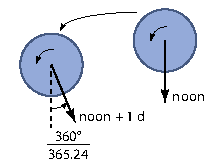
\includegraphics[width=\linewidth]{solar-day}
\caption[The movement of the Earth from noon to noon]{The movement of the Earth from noon to noon.  The arrows indicate the direction towards the Sun.}
\label{f.solar-day}
\end{marginfigure}

There are $365.24$ solar days between successive solar crossings of the vernal equinox, which defines a \emph{tropical year}.  Over the course of this year, the extra rotation on each solar day adds up to one complete rotation of the Earth.  The Earth rotates $366.24$ times in one tropical year, and therefore the rotation period of the Earth is
\[ \frac{365.24}{366.24}\times \val{24}{\hour} =  \hrangle{23}{56}{04}.  \]
In fact, the tropical year is slightly shorter, by about $\val{20}{\minute} = \val{1}{\yr}/26\,000$ because of the precession of the Earth's axis.

Our time---hours and minutes---is tied to the position of the Sun, which is convenient for daily activity but not so convenient if we want to know when a particular star is observable.  Instead of marking when the Sun crosses our meridian, we define our local \emph{sidereal time} relative to our meridian crossing the vernal equinox.  Because we also define right ascension relative to the vernal equinox, objects with a right ascension near that of the sidereal time will be high in the sky.

To compute our local sidereal time, first determine the right ascension of the Sun (Exercise \ref{ex.RA-sun}); this will then fix the offset between the local sidereal time and the local noon in UTC.  We can then compute our offset for local noon based on our longitude.

\begin{exercisebox}[Current sidereal time]
Local noon at $0^{\circ}$ longitude corresponds to 12:00 UTC. Given that our longitude is $\dec{84}{28}{33}\,\mathrm{W}$, what is our local noontime in UTC.  What local time would this correspond to today? From this and your estimate of the Sun's current hour angle, what is the current sidereal time?
\end{exercisebox}

\section{Parallax}

The motion of the Earth around the Sun \emph{does} cause a small shift in the apparent angular position of a star, a phenomena known as \emph{parallax}.  This effect is exploited to determine the distance to nearby stars.  

\begin{figure*}[htb]
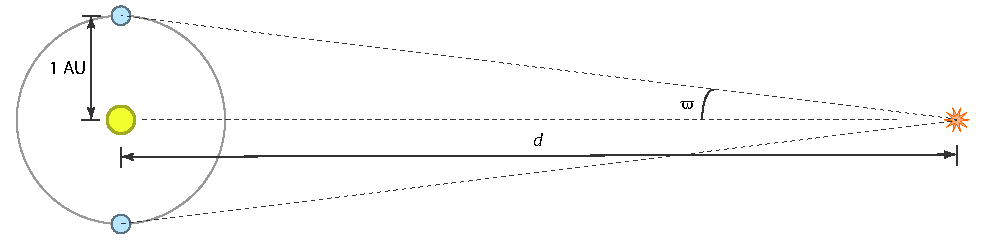
\includegraphics[width=\linewidth]{parallax}
\caption[The parallax angle of a star]{The parallax angle $\varpi$ of a star induced by Earth's motion around the Sun.}
\label{f.parallax}
\end{figure*}

The angular shift, $\varpi$, is related (see Fig.~\ref{f.parallax}) to the radius of the Earth's orbit, \val{1}{\AU}, and the distance to the star $d$ via
\[
\frac{\val{1}{\AU}}{d} = \tan\varpi \approx \varpi.
\]
When $\varpi$ is expressed in arcseconds, this gives
\begin{equation}\label{e.parallax}
d = \frac{\val{206\,265}{\AU}}{\varpi/1''} = \val{1}{\parsec}\left(\frac{1''}{\varpi}\right) ,
\end{equation}
which defines the \emph{parsec}.  In CGS units $\val{1}{\parsec} = \val{\sci{3.086}{18}}{\cm}$, which is a bit over 3 light-years.

\section{Angular distances between nearby objects}

To compute the angular distance between two points on the sky, we draw two vectors $\bvec{a}$, $\bvec{b}$ to these points and use
\[ \cos\theta = \frac{\bvec{a}\vdot\bvec{b}}{|\bvec{a}||\bvec{b}|}. \]
Since both $\bvec{a}$ and $\bvec{b}$ lie on the unit sphere, $|\bvec{a}| = |\bvec{b}| = 1$; the $(x,y,z)$ components of these vectors are
\[
\left(\cos\delta_{1}\cos\eta_{1}, \cos\delta_{1}\sin\eta_{1}, \sin\delta_{1}\right)
\]
and
\[
\left(\cos\delta_{2}\cos\eta_{2}, \cos\delta_{2}\sin\eta_{2}, \sin\delta_{2}\right),
\]
respectively. 
Taking the dot product,
\begin{eqnarray}
\cos\theta &=& \cos\delta_{1}\cos\delta_{2}\left(\cos\eta_{1}\cos\eta_{2} + 
	\sin\eta_{1}\sin\eta_{2}\right) + \sin\delta_{1}\sin\delta_{2}\nonumber\\
	 &=& \cos\delta_{1}\cos\delta_{2}\cos\left(\eta_{1}-\eta_{2}\right) + 
	 	\sin\delta_{1}\sin\delta_{2}.
\label{e.angular-distance}
\end{eqnarray}

\begin{marginfigure}[-14\baselineskip]
\includegraphics[width=\linewidth]{angular-distance}
\caption[Angular distance between two points on a sphere]{Two locations on the sphere separated by a distance $\theta$.}
\label{f.angular-distance}
\end{marginfigure}

We are usually interested in the angular distance between two nearby sources, with RAs $\eta_{1} \approx \eta_{2}$ and declinations\sidenote{Notice our coordinates differ from the usual spherical polar coordinates: $\delta$ is measured from the $x$-$y$ plane, not from the $z$-axis.} $\delta_{1}\approx\delta_{2}$.  We can use the expansion rule,
\[ \cos x \approx 1 - \frac{x^{2}}{2},\qquad x \ll 1 \, \]
on $\theta$ and $\eta_{1}-\eta_{2}$ in equation~(\ref{e.angular-distance}):
\begin{eqnarray*}
	1-\frac{\theta^{2}}{2} &\approx& \cos\delta_{1}\cos\delta_{2} \left[1-\frac{(\eta_{1}-\eta_{2})^{2}}{2}\right] + \sin\delta_{1}\sin\delta_{2}\\
		&=& \cos(\delta_{1}-\delta_{2}) - \cos\delta_{1}\cos\delta_{2}\frac{(\eta_{1}-\eta_{2})^{2}}{2}.
\end{eqnarray*}
\marginnote[-5\baselineskip]{%
We make heavy use of the sine and cosine addition formula: $\cos(x+y) = \cos x\cos y - \sin x\sin y$, and $\sin(-y) = -\sin y$, $\cos(-x) = \cos(x)$.}
We can now expand $\cos(\delta_{1}-\delta_{2})$, cancel common factors and multiply by 2,
\[ \theta^{2} \approx (\delta_{1}-\delta_{2})^{2} + \cos\delta_{1}\cos\delta_{2}(\eta_{1} - \eta_{2})^{2}. \]
Finally, we notice that to lowest order, $\cos\delta_{1}\cos\delta_{2}\approx \cos^{2}\delta$, where $\delta = (\delta_{1}+\delta_{2})/2$ is the average of the two declinations.  This gives us a formula for the angular distance $\theta$ between two nearby points,
\begin{equation}
\theta \approx \sqrt{\cos^{2}\delta\left(\eta_{1}-\eta_{2}\right)^{2} + \left(\delta_{1}-\delta_{2}\right)^{2}}.
\end{equation}
This looks like the pythagorean formula; the factor of $\cos\delta$ accounts for the lines of constant RA converging as they approach the poles.

\begin{marginfigure}[12\baselineskip]
\includegraphics[width=\linewidth]{angular-distance2}
\caption[Angular distance between lines of constant right ascension]{The distance between two RAs $\eta_{1}$ and $\eta_{2}$, measured along a circle of radius $\cos\delta$.}
\label{f.angular-pythagorean}
\end{marginfigure}

\begin{exercisebox}[Angular size of the Pleiades]
Atlas A and Electra are two bright stars that lie on the east and west sides of the Pleiades star cluster.  Atlas has right ascension $\RA = \hrangle{03}{49}{09.7}$ and declination $\delta = \dec{24}{03}{12}$; Electra has $\RA = \hrangle{03}{44}{52.5}$ and $\delta = \dec{24}{06}{48}$.  Find the angular distance between these stars.  If the distance to the Pleiades is $\val{136}{\parsec}$, what is the projected distance between these stars?
\end{exercisebox}

\section{Looking up}
Finally a note about directions when looking up at the sky.  We've drawn our coordinates from the perspective of someone outside the celestial sphere; our perspective, however, is from the center.  When we look up at the sky, if we face south, so that the direction northwards is at the top of our field of view, then the easterly direction is to our \emph{left}. Objects of larger right ascension are therefore to our left as well.

% %!TEX root = ../planets-notes.tex

What do we actually measure when we observe a star? A star emits photons with a range of wavelengths over the electromagnetic spectrum.  The total emitted energy per second over all wavelengths is the star's \newterm{luminosity}.  For example, the solar luminosity is $\Lsun = \val{\sci{3.86}{26}}{\unitstyle{W}}$.  A telescope collects only a small fraction of this power: if a telescope has a collecting area $\mathcal{A}$ and is a distance $d$ from the star, then it intercepts a fraction $\mathcal{A}/(4\pi d^{2})$ of the star's light.  We call $F = L/(4\pi d^{2})$ the \newterm{flux}. The units of flux are $\unitstyle{W}\,\meter^{-2}$.

More specifically, $F$ is the \newterm{bolometric flux}, that is, the flux over all wavelengths.  Of course, no telescope detects \emph{all} wavelengths of light. Many wavebands, e.g., UV, X-ray, and infrared, do not even penetrate the Earth's atmosphere.  Moreover, detectors (photographic plates or CCD's) are not uniformly efficient at converting photons into a signal.

In order to have a common standard, (optical) astronomers use \newterm{filters}, which transmit light only in certain wavelength bands. In this context, the flux refers to the power per area carried by light with wavelengths in that band.  For historical reasons, astronomers define \newterm{magnitudes}, which are a relative logarithmic\sidenote{In these notes, $\lg\equiv\log_{10}$ and $\ln\equiv\log_{e}$.} scale for fluxes.  The difference in magnitude between two stars is defined by
\begin{equation}\label{e.magnitude-def}
	m_{1} - m_{2} = -2.5\lg\left(\frac{F_{1}}{F_{2}}\right)
\end{equation}
where the magnitudes $m_{1}$, $m_{2}$ and fluxes $F_{1}$, $F_{2}$ refer to light that has been passed through a particular filter.

\begin{margintable}
\label{t.ubvr}\caption{Selected common filters about the range of visible wavelengths \citep{Binney1998Galactic-Astron}.  Here ``FWHM'' means ``Full width at half-maximum.''}
\begin{tabular}{lrr}
\hline
Filter & $\lambda_{\mathrm{eff}}/\nano\meter$ & FWHM/nm \\
\hline\hline
U & 365 &  66\\
B & 445 &  94\\
V & 551 &  88\\
R & 658 & 138\\
\hline
\end{tabular}
\end{margintable}

Note that magnitudes are defined as the ratio of two fluxes. This is very useful when comparing the relative brightness of two stars; unfortunately it makes conversion to a physical unit ($\unitstyle{W}\usk\meter^{-2}\usk\nano\meter^{-1}$) non-trivial.  The magnitude scales are typically defined so that the star Vega has $U=B=V=\ldots=0$.\sidenote{But for historical reasons, $V(\textrm{Vega}) = +0.04.$}


\newpage
\begin{exercisebox}[Relation between magnitude and flux]
\begin{enumerate} 
\item Suppose we have two identical stars, A and B. Star A is twice as far away as star B. What is $m_{A} - m_{B}$?
\item Suppose a star's luminosity changes by a tiny amount $\delta$.  What is the corresponding change in that stars' magnitude?
\end{enumerate}
\end{exercisebox}

\newthought{If we take a ratio of two magnitudes using different filters from a single star,} then we have a rough measure of the star's color.  This ratio is called a \newterm{color index}.  For example, 
\[ B - V \equiv m_{B} - m_{V} = -2.5\lg\frac{F_{B}}{F_{V}} \]
gives a measure for how blue the star's spectrum appears.

\begin{exercisebox}[The $B-V$ index]
Which has the larger $B-V$ index: a red star, like Betelgeuse, or a blue-white star, like Rigel?
\end{exercisebox}

\newthought{Two stars with the same apparent brightness} may have very different intrinsic brightnesses: one may be very dim and nearby, the other very luminous and faraway.  To compare intrinsic brightness, we need to correct for the distance to the star\sidenote{This assumes we \emph{know} the distance, which can be difficult!}.  We define the \newterm{distance modulus} as the difference in magnitude between a given star and the magnitude it would have if it were at a distance of \val{10}{\parsec}:
\begin{eqnarray*}
 \mathrm{DM} \equiv m - m(\val{10}{\parsec}) &=& -2.5\lg\left[\frac{L}{4\pi d^{2}} \frac{4\pi (\val{10}{\parsec})^{2}}{L}\right] \\
 	&=& -2.5\lg\left(\frac{\val{10}{\parsec}}{d}\right)^{2} \\
	&=& 5\lg\left(\frac{d}{\parsec}\right) - 5.
\end{eqnarray*}
The magnitude that the star would have if it were at \val{10}{\parsec} distance is called its \newterm{absolute magnitude}, $M \equiv m - \mathrm{DM}$.

\section{Light is a wave}

\begin{marginfigure}
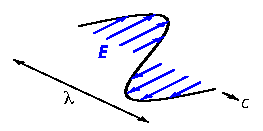
\includegraphics[width=\linewidth]{light-wave}
\caption[The electric force in a light wave]{Schematic of the electric force (blue arrows) for a wave traveling towards us at speed $c$ with wavelength $\lambda$.}
\label{f.light-wave}
\end{marginfigure}
Charges feel an electric force.
When we detect light, what happens at the atomic level is that the charges in our detector (antenna, CCD, eye) feel an electric force that oscillates with frequency $\nu$. If we could set up a grid of detectors and measure the electric force per unit charge, we would notice a sinusoidal pattern traveling at speed\sidenote{This velocity is exact; the meter is defined in terms of the speed of light.} $c = \val{299\,792\,458}{\meter/\second}$ with a wavelength $\lambda = c/\nu$.  We call this force per charge the electric field $\bvec{E}(\bvec{x},t)$. The \newterm{intensity} of the light at our detector is proportional to $|\bvec{E}|^{2}$.

In situations in which the wavelength is small (relative to the system in question), light propagates along rays.  The rule for propagation is known as \newterm{Fermat's principle:} the path is that for which the propagation time is minimized. To illustrate this, we shall use it to derive the laws for reflection and refraction.

Consider light reflecting from a mirror as shown in the top panel of Figure~\ref{f.reflection-and-snell}. The time for light to propagate from source to observer is
\[	\tau = \frac{1}{c}\left[\sqrt{h_{s}^{2}+x^{2}} + \sqrt{h_{o}^{2} + (w-x)^{2}}\right]. \]
To minimize the path length, we compute $\dif\tau/\dif x$ and set it to zero,
\[
	0 = \DD{\tau}{x} = \frac{1}{c}\left[\frac{x}{\sqrt{h_{s}^{2}+x^{2}}} 
	- \frac{w-x}{\sqrt{h_{o}^{2} + (w-x)^{2}}}\right] = \frac{1}{c}\left[\sin i - \sin r\right].
\]
Hence the light travels such that $i = r$: the angles of incidence and reflection are equal.

\begin{marginfigure}
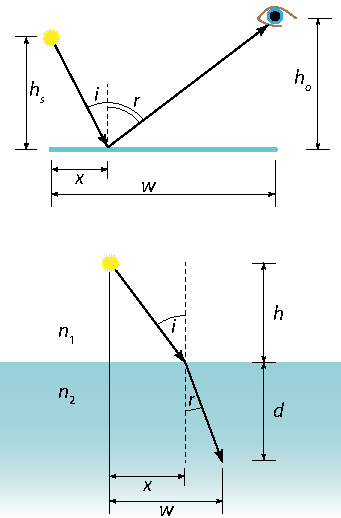
\includegraphics[width=\linewidth]{reflection-and-snell-AST208}
\caption[Reflection and refraction]{Top: reflection of light from a surface. Bottom: refraction of light as it passes from a medium with index $n_{1}$ into a medium with index $n_{2}$.
\label{f.reflection-and-snell}}
\end{marginfigure}

For a second example, consider the passage of light from one medium to another, as depicted in the bottom panel of Figure~\ref{f.reflection-and-snell}.  The interaction of matter with the oscillating electric field causes the light to travel at a speed $c/n$, where $n$ is called the \newterm{index of refraction} and is a property of the material. For the situation in Fig.~\ref{f.reflection-and-snell}, the propagation time is
\[
	\tau = \frac{n_{1}}{c}\sqrt{h^{2}+x^{2}} + \frac{n_{2}}{c}\sqrt{d^{2} + (w-x)^{2}};
\]
minimizing the propagation time with respect to $x$ gives
\[
	0 = \frac{n_{1}}{c}\frac{x}{\sqrt{h^{2}+x^{2}}} - \frac{n_{2}}{c} \frac{w-x}{\sqrt{d^{2} + (w-x)^{2}}} = \frac{1}{c}\left[ n_{1}\sin i - n_{2} \sin r \right].
\]
This result, $n_{1}\sin i = n_{2}\sin r$, is also known as \newterm{Snell's law}.

\begin{marginfigure}[5em]
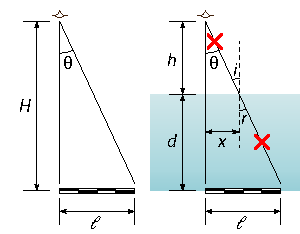
\includegraphics[width=\linewidth]{magnification-in-water}
\caption{Change in angular size of an object in water.
\label{f.magnification-in-water}}
\end{marginfigure}
\begin{exercisebox}[Magnification of an object in water]
A small stick of length $\ell$ is placed on the bottom of an empty swimming pool as shown in Fig.~\ref{f.magnification-in-water}; when you look down on the stick from a height $H$ above the bottom of the pool, the stick subtends an angle $\tan\theta = \ell/H$.  The pool is then filled with water ($n=4/3$) to a depth $d$.  Because of refraction, the stick will appear to subtend a different angle $\theta'$.  Correct the right hand diagram of Fig.~\ref{f.magnification-in-water} to show how the light ray propagates from the ends of the stick to your eye.  Is $\theta'$ larger or smaller than $\theta$---is the image of the stick magnified or reduced?  For the case $\ell \ll H$, so that $\theta \ll 1$, use the small angle expansions to derive an expression $\theta' = 
\theta \mathcal{M}$, where $\mathcal{M}$ depends on $h$, $d$, and $n$.
\end{exercisebox}

\section{Diffraction}

A telescope makes an image by focusing the incoming rays of light onto a detector.
Suppose we are at a fixed point and the wave is propagating past us.  In general we would observe an electric field amplitude of the form 
\[ E(t) = A_{0}\cos\left(2\pi \nu t \right)  + B_{0}\sin\left(2\pi \nu t \right) \]
where $\nu = c/\lambda$ is the frequency.  Let's check this: in going from $t=0$ to $t=T=1/\nu$, the period of the wave, the argument of the cosine and sine goes from $0$ to $2\pi$, which is one oscillation.  To find the net intensity $I$ from a number of waves, we sum the amplitudes to get the net electric field $\bvec{E}$ and then take the square $|\bvec{E}|^{2}$.

Now imagine the electromagnetic wave incident on our telescope. The source is very distant, so the wavefront (a surface of constant phase) is a plane---think of sheets of paper moving downward onto the telescope.  To make an image, the telescope focuses the incident radiation to a point on the detector. There is a limit, however, to how sharply the image can be focused.  Let's look at a small angle $\theta$ away from the axis.  Then the wavefront is incident on the telescope as shown in Figure~\ref{f.diffraction}. To keep the math tractable, we'll make our telescope opening one-dimensional and we'll break it into a $N+1$ little detectors spaced a distance $d = D/N$ apart.

\begin{figure}[hb]
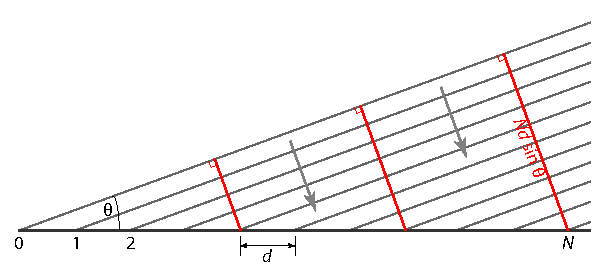
\includegraphics[width=\linewidth]{diffraction}
\caption[A plane wave incident on a detector]{Schematic of a plane wave incident at angle $\theta$ on a detector.}
\label{f.diffraction}
\end{figure}

Because of the angle, the light travels an extra distance $d\sin\theta$ to reach detector 1, $2d\sin\theta$ to reach detector 2, and so on.  As a result, if the phase at the first detector (number 0) is $\chi$, the phase at detector 1 is $\chi + 2\pi d\sin\theta/\lambda$, at detector 2,  $\chi + 4\pi d\sin\theta/\lambda$, and so on.  When we combine the signals from these detectors, the amplitude of the electric field will have the form
\begin{eqnarray*}
E &=& A_{0}\left[\cos\chi + \cos\left(\chi + 2\pi\frac{d\sin\theta}{\lambda}\right)
	+ \cos\left(\chi + 2\pi\frac{2d\sin\theta}{\lambda}\right) + \right.\\
	&&	+ \left.\cos\left(\chi + 2\pi\frac{3d\sin\theta}{\lambda}\right) + \ldots 
	+ \cos\left(\chi + 2\pi\frac{Nd\sin\theta}{\lambda}\right)\right]\\
	&& + B_{0}\left[ \sin\chi + \sin\left(\chi + 2\pi\frac{d\sin\theta}{\lambda}\right) 
		+ \ldots + \sin\left(\chi+2\pi\frac{Nd\sin\theta}{\lambda}\right)\right].
\end{eqnarray*}
When $\theta \to 0$, the amplitude goes to $E \to (N+1)\left[A_{0}\cos\chi + B_{0}\sin\chi\right]$, and so the brightness $I(\theta\to 0) = |E|^{2}$ is a very large number.  That's good: the light from the star is focused to a point. Now, how large does $\theta$ have to be before $E$ goes to zero?

To find this, let's first set $\chi = 0$ to keep things simple. There are a number of ways to find the sum; a particularly easy way is to recognize that this sum over cosines looks like adding up the $x$-component of vectors, and the sum over the sines looks like adding the $y$-component of vectors.  We add the vectors by placing them nose-to-tail as shown in Fig.~\ref{f.vector-addition}.  The net amplitude is then $A_{0}$ times the $x$-component of the red vector, plus $B_{0}$ times the $y$-component of the red vector.  Clearly if we want both the sum over sines and over cosines to vanish, we need the vectors to make a complete circle.

\begin{marginfigure}
\centering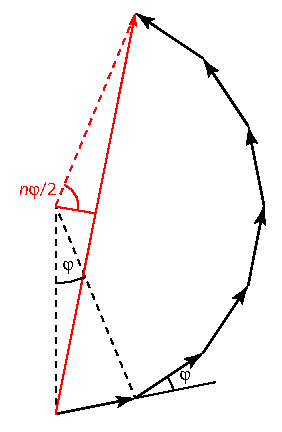
\includegraphics[width=0.8\linewidth]{vector-addition}
\caption[Addition of vectors with phase differences]{Addition of a series of vectors with a phase difference $\phi$.}
\label{f.vector-addition}
\end{marginfigure}

In this addition, each vector has length 1. If $N+1$ is large, then the circumference of the circle is approximately $(N+1) = 2\pi r$.  For small $\phi = (2\pi d/\lambda)\sin\theta$, the radius of the circle is $r \approx 1/\phi$.  Hence the condition for our vectors to sum to zero becomes
\[ N+1 = \frac{2\pi}{\phi} = \frac{2\pi\lambda}{2\pi d\sin\theta} \]
Now, we assume that $N \gg 1$, so that $(N+1)d \approx Nd = D$, the diameter of our telescope's aperture.  Then, the brightness falls to zero an angle
\[ \sin\theta \approx \theta \approx\lambda/D\]
away from the center of the star's image.

The full form of the intensity as a function of angle from the beam axis is,
\begin{equation}\label{e.intensity-diffraction}
I = I_{0}\left[\frac{\sin\left(\pi D/\lambda\,\sin\theta\right)}{\sin\left(\pi d/\lambda\,\sin\theta\right)}\right]^{2}.
\end{equation}

\begin{exercisebox}[Diffraction of image of a point source]
Write a \code{Python} function that computes eq.~(\ref{e.intensity-diffraction}) for different values of $N$ and $D/\lambda$.  Plot $I/(I_{0}n^{2})$ against $\theta\lambda/D$.  Describe your findings.
\end{exercisebox}

The wave nature of light places a limitation on the \newterm{resolving power} of a telescope, defined as the   angular separation for which two point sources can be distinguished.  Two point-like objects separated by an angular distance $\lesssim \lambda/D$ will have their images smeared into one.

\begin{exercisebox}[Resolving power of various instruments]
What is the resolving power of the \emph{Hubble Space Telescope} ($D=\val{2.4}{\meter}$) and the Keck telescope ($D=\val{10}{\meter}$) at a wavelength $\lambda = \val{570}{\nano\meter}$? Estimate the angular resolution of the human eye at that wavelength. What is the resolving power of the Arecibo radio telescope ($D = \val{305}{\meter}$) at a frequency of \val{3}{\Giga\Hz}?
\end{exercisebox}

For ground-based telescopes, an even more severe limitation is the refraction of light by the atmosphere. The atmosphere is turbulent, and the swirling eddies contain variations in density that change the refractive index and distort the wavefront.  This distortion smears the image over an angular scale that is typically larger than $1''$.

\begin{exercisebox}[Angular size of star, planet]
What is the angular size of a solar-sized star ($\Rsun = \val{\sci{6.96}{5}}{\kilo\meter}$) at a distance of $\val{1}{\parsec}$?  What is the angular size of Mars ($R_{\mars} = \val{3\,390}{\kilo\meter}$) at a distance of $\val{0.5}{\AU}$?  How would the difference in angular size affect the appearance of these two objects?
\end{exercisebox}

\newthought{In addition to distorting the wavefront, the air also attenuates the brightness of the light.} The amount of attenuation depends on the column, that is, the mass per unit area of air along the line of sight, which in turn depends on the viewing angle (Fig.~\ref{f.airmass}).

\begin{marginfigure}
\includegraphics[width=\linewidth]{airmass}
\caption[Illustration of airmass]{Illustration of the greater column of atmosphere (airmass) that the light from a star an angle $z$ from the zenith must traverse.}
\label{f.airmass}
\end{marginfigure}

Astronomers define the \newterm{airmass} $m$ as a function of zenith angle $z$ by
\[
	\textrm{air mass} = \frac{\int\rho(r)\,\dif \ell}{\int\rho(r)\,\dif r}
\]
where $\ell$ is along the line of sight to the star.  For a planar atmosphere, $\dif\ell = \dif r/\cos z = \sec z\,\dif r$, and so the airmass is just $\sec z$.  The dimming of the star is proportional to $\exp\left[-\int\rho(r)\,\dif\ell\right]$, and therefore the magnitude of a star at zenith angle $z$ varies as
\[ m(z) = k \sec z + c, \]
where $k$ and $c$ are constants.  By measuring the apparent brightness of the star at several different zenith angles, astronomers can empirically determine these constants.

% %!TEX root = ../AST208-notes.tex

\section{The Difficulty with Direct Detection}

Suppose we want to observe exoplanets directly. Let's first estimate how far we have to look.  

\begin{exercisebox}[Mean distance to star in a sample]
\label{e.mean-distance}
The density of stars in the solar neighborhood is $\val{0.14}{\parsec^{-3}}$.  Suppose 50\% of the stars have planets, and we want a sample of about 20 planetary systems.  What would be the radius (in parsec) of the volume containing this many systems?  Given this radius, what is the average distance to a star in this sample?
\end{exercisebox}

Next let's estimate the difference in brightness between a planet and its host star. We shall use our solar system as an example.

\begin{exercisebox}[Ratio of flux from planet, star]
The Sun, which is at a distance of $\val{1}{\AU}$, has an apparent $V$-band magnitude $V_{\odot} = -26.74$.  At its closest approach of approximately $\val{4}{\AU}$, Jupiter has an apparent magnitude $V_{\jupiter} = -2.94$.  Compute the ratio of fluxes in $V$-band, i.e., $F_{\jupiter}/F_{\odot}$, if both Jupiter and the Sun were at the same distance.
\end{exercisebox}

Finally, we know that there is a limit to the angular resolution of a telescope. This limit is imposed by both the atmospheric seeing and the telescope optics.  Let's estimate how the angular separation of planet and star compares with a fiducial angular resolution.

\begin{exercisebox}[Resolving planets]
Jupiter's mean distance from the Sun is $\val{5.2}{\AU}$. Suppose we were to view the Sun-Jupiter system from the average distance derived in exercise \ref{e.mean-distance}; what would be the angular separation between Jupiter and the Sun?  How does this compare with the atmospheric seeing under good conditions?
\end{exercisebox}

As these exercises illustrate, imaging a planet directly is a daunting task. Astronomers have therefore resorted to indirect means, in which the host star is observed to vary due to the influence of the planet's gravitational force. This motivates a review of Kepler's problem.

\section{Planetary Orbits: Kepler}

Suppose we have a exoplanet system with a planet $p$ and a star $s$.  The vector from the star to the planet is $\rv_{sp} = \rv_{p}-\rv_{s}$, and the force that the star exerts on the planet is
\begin{equation}\label{e.newton}
	\bvec{F}_{sp} = -\frac{GM_{p}M_{s}}{|\rv_{sp}|^{3}} \rv_{sp}.
\end{equation}
The planet exerts a force on the star $\bvec{F}_{ps} = -\bvec{F}_{sp}$.

To make this problem more tractable, we shall put the origin of our coordinate system at the center of mass, as shown in Fig.~\ref{f.center-mass},
\begin{marginfigure}
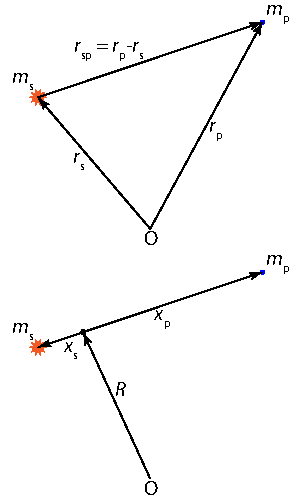
\includegraphics[width=\linewidth]{center-of-mass}
\caption[Center of mass]{Center of mass in a star-planet system.}
\label{f.center-mass}
\end{marginfigure}
\[ \bvec{R} = \frac{M_{s}\rv_{s} + M_{p}\rv_{p}}{M_{s}+M_{p}}; \]
in this frame the star and planet have positions 
\begin{eqnarray}
 \xv_{s} &=& \rv_{s}-\bvec{R} = -\frac{M_{p}}{M_{p}+M_{s}}\rv_{sp}\label{e.star-pos}\\
 \xv_{p} &=& \rv_{p}-\bvec{R} = \frac{M_{s}}{M_{p}+M_{s}}\rv_{sp}\label{e.planet-pos}
\end{eqnarray}
and hence accelerations
\begin{eqnarray*}
 \DDtt{\xv_{s}} &=& -\frac{M_{p}}{M_{p}+M_{s}}\DDtt{\rv_{sp}} \\
 \DDtt{\xv_{p}} &=& \frac{M_{s}}{M_{p}+M_{s}}\DDtt{\rv_{sp}}.
\end{eqnarray*}

If we substitute this acceleration into the equation of motion for the planet,
\[ M_{p}\DDtt{\xv_{p}} = \bvec{F}_{sp}, \]
and use eq.~(\ref{e.newton}) for $\bvec{F}_{sp}$, we get the reduced equation of motion
\begin{equation}\label{e.one-body}
 \DDtt{\rv_{sp}} = -G\frac{M_{s}+M_{p}}{|\rv_{sp}|^{3}} \rv_{sp}.
\end{equation}
We recover this same equation if we substitute the accelerations into the equation of motion for the star. Hence for a two body problem, we only need to solve equation~(\ref{e.one-body}) for $\rv_{sp}(t)$ and then use equations~(\ref{e.star-pos}) and (\ref{e.planet-pos}) to compute the positions $\xv_{s}(t),\xv_{p}(t)$ of the star and planet.

\begin{exercisebox}[Center-of mass for Sun-Jupiter]
Locate the center of mass for the Sun-Jupiter system:
\[ \frac{\Msun}{M_{\mathrm{\jupiter}}} = 1047; \qquad \rv_{\mathrm{\odot\jupiter}} = \val{5.2}{\AU}. \]
\end{exercisebox}

The solution to equation~(\ref{e.one-body}) is an elliptical orbit (Fig.~\ref{f.elliptical-orbit}) with the center-of-force at one focus of the ellipse.  The period $T$ depends on the semi-major axis $a$ of the ellipse,
\begin{equation}\label{e.period}
	T^{2} = \frac{4\pi^{2}}{G(M_{s}+M_{p})} a^{3}.
\end{equation}
Suppose the orbit is circular, so that $|\rv_{sp}|=a$ is constant.  Then by combining equations~(\ref{e.period}) and (\ref{e.star-pos}) we can find the orbital speed of the star,
\begin{equation}\label{e.star-velocity}
	v_{s} = \frac{M_{p}}{M_{s}+M_{p}} \times \frac{2\pi a}{T} = \left[\frac{GM_{p}}{a}
	\frac{M_{p}}{M_{s}+M_{p}}\right]^{1/2}.
\end{equation}
This speed is detectable via doppler shift of the stellar absorption lines.

\begin{marginfigure}
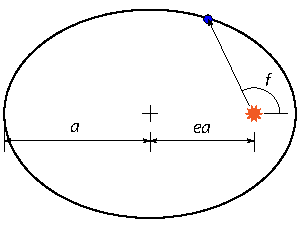
\includegraphics[width=\linewidth]{elliptical-orbit}
\caption[Orbital elements]{Orbital elements for a body moving in a gravitational potential about a fixed center of force, indicated by the yellow star.}
\label{f.elliptical-orbit}
\end{marginfigure}

\begin{exercisebox}[Orbital speed of the Sun]
\label{ex.sun-orbital-speed}
	Compute the orbital speed of the Sun for the two-body Sun-Jupiter system;
\[ \frac{\Msun}{M_{\mathrm{\jupiter}}} = 1047; \qquad \rv_{\mathrm{\odot\jupiter}} = \val{5.2}{\AU}. \]
\end{exercisebox}

\begin{exercisebox}[Doppler shift of Sun]
	What is the wavelength shift induced by the motion of the Sun, computed in exercise \ref{ex.sun-orbital-speed}, for an absorption line with rest wavelength $\val{600}{\nano\meter}$?
\end{exercisebox}

\section{Transits}

In \S~\ref{s.doppler} we derived the doppler shift for motion along our line-of-sight.
In general, however, the orbit is not edge-on, but rather inclined at an angle (Fig.~\ref{f.orbital-inclination}).
In this case the speed that is measured via doppler shift of stellar lines is $v_{s}\sin i$.  Thus, our problem becomes, given a measurement of period $T$ and projected speed $K = v_{s}\sin i$, what can we learn about the planet?

\begin{figure}[ht]
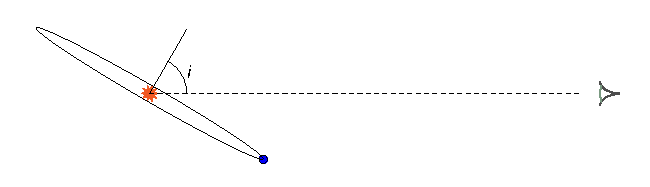
\includegraphics[width=\linewidth]{orbital-inclination}
\caption[Schematic of the inclination of a planetary orbit]{Schematic of the inclination of a planetary orbit to our line of sight.}
\label{f.orbital-inclination}
\end{figure}

We can combine equations~(\ref{e.period}) and (\ref{e.star-velocity}) into the form
\begin{equation}\label{e.mass-fcn}
	\frac{M_{p}^{3}\sin^{3}i}{(M_{s}+M_{p})^{2}} = \frac{K^{3}T}{2\pi G}.
\end{equation}
The right-hand side is in terms of the observed quantities $K$ and $T$, and is therefore determined from observations.  We expect $M_{s} \gg M_{p}$, and can usually estimate $M_{s}$ from spectroscopy of the star.  Even with this information, we can only determine $M_{p}\sin i$.

For systems with sufficiently large inclination, we will observe the planet to \emph{transit} the star, that is, to pass in front of the stellar disk. From Fig.~\ref{f.transit}, if
\begin{marginfigure}
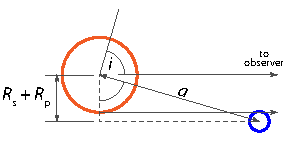
\includegraphics[width=\linewidth]{transit}
\caption[Schematic of a planetary transit]{Schematic of a planetary transit.}
\label{f.transit}
\end{marginfigure}
\[	\cos i < \frac{R_{s}+R_{p}}{a},	\]
then the light from the star will be partially blocked during some part of the orbit.\sidenote{We are assuming that the star is sufficiently far away that we can ignore the angle subtended by the star.}

\begin{exercisebox}[Inclination required to observe transit]
For the Sun-Jupiter system ($\Rsun = \val{\sci{6.96}{5}}{\kilo\meter}$, $R_{\jupiter}=\val{71\,400}{\kilo\meter}$, $a = \val{5.2}{\AU}$), what orbital inclination is required for an observer in a distant planetary system to witness a transit?
\end{exercisebox}

\newthought{What is the probability distribution of a star's inclination?}
To derive this, let's imagine each planet's orbital angular momentum as a vector having unit length.  We don't care about whether, from out perspective, the planet orbits counterclockwise or clockwise, so we put all of the arrows with $0\le i\le \pi/2$, as shown in figure~\ref{f.inclination-probability}.  

\begin{figure}[ht]
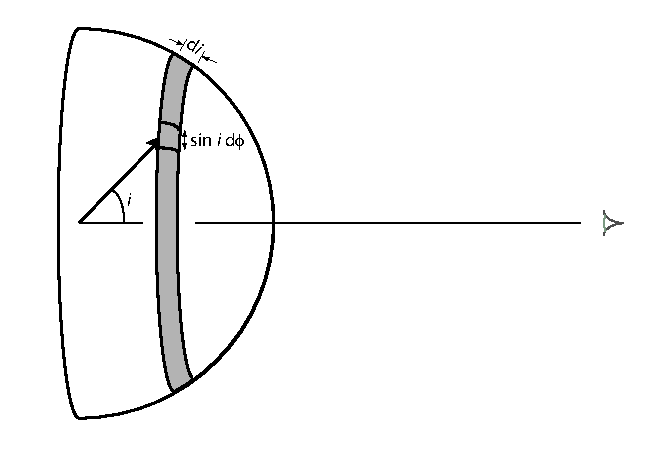
\includegraphics[width=\linewidth]{inclination-probability}
\caption[Schematic of the probability distribution of orbital inclination]{Schematic of the probability of the orbital inclination lying within $(i,i+\dif i)$ and $(\phi,\phi+\dif\phi)$.}
\label{f.inclination-probability}
\end{figure}

Now imagine a huge sample of planetary systems.  If the orbits are randomly distributed, then we expect the arrows to be evenly distributed over our hemisphere; as a result, the probability of a planet having inclination in $(i,i+\dif i)$ and azimuthal angle in $(\phi,\phi+\dif\phi)$ is the ratio of the area of that little coordinate patch to the area of the hemisphere,
\[ p(i,\phi)\,\dif i\,\dif \phi = \frac{\sin i\,\dif i\,\dif\phi}{2\pi}. \]
Since we aren't interested in the azimuthal angle, we can integrate over $\phi$ to find the probability distribution for a planet to have a given inclination, $p(i) = \sin i$.


\begin{exercisebox}[Mass-function and distribution of masses]
From a solar-mass star you measure a periodic doppler shift with $T = \val{3}{\yr}$ and $K = \val{18}{\meter\usk\second^{-1}}$.  What is the probability that the planet has a mass $>\val{2}{M_{\jupiter}}$? What is the probability that the planet has a mass $>\val{10}{M_{\jupiter}}$?
\end{exercisebox}

\begin{exercisebox}[Fraction of orbit in transit]
\begin{enumerate}\renewcommand{\labelenumi}{\alph{enumi})}
\item\label{e.transit-fraction}
For an edge-on, circular orbit, show that the fraction of the orbit during which the planet is in transit is
\[ f = \frac{T_{\mathrm{tr}}}{T} = \frac{R_{s}+R_{p}}{\pi a}, \]
where $a$ is the orbital separation.

\item\label{e.transit-duration}
Derive an expression for the transit duration $T_{\mathrm{tr}}$ in terms of $a$ and the masses and radii of the star and planet.

\item\label{e.transit-properties-jupiter}
For the Sun-Jupiter system, what is $f$ and $T_{\mathrm{tr}}$?

\end{enumerate}
\end{exercisebox}


% %!TEX root = ../AST208-notes.tex
\chapter{Beyond Kepler's Laws}

\section{Motion in a rotating frame}

\begin{marginfigure}
\includegraphics[width=\linewidth]{polar-coordinates}
\caption[Polar coordinates]{Polar coordinates for a particle.
\label{f.polar-coordinates}}
\end{marginfigure}
To work out the equations of motion in a rotating frame, we start from an inertial frame in polar coordinates.  In this system, the particle is located at $(r,\theta)$; the position vector of the particle is $\rv = r\rhat$. After an internal $\Delta t$, the particle's position is $(r+\Delta r,\theta+\Delta\theta)$, as shown in Fig.~\ref{f.polar-coordinates}.  

As the particle moves, both $\rhat$ and $\thetahat$ change as well.  Since both $\rhat$ and $\thetahat$ are unit vectors, only their direction changes with their magnitude remaining constant. Neither vector changes under purely radial motion, $\Delta\theta = 0$.  Under a change in angle, $\Delta\theta$, both $\rhat$ and $\thetahat$ rotate by an angle $\Delta\theta$, as shown in Fig.~\ref{f.change-polar-unit-vectors}. In the limit $\Delta\theta \to 0$, 
\[ \Delta \rhat \to \Delta\theta \thetahat; \quad \Delta\thetahat \to -\Delta\theta\rhat. \]
Dividing by $\Delta t$ and calling $\omega = \dif\theta/\dif t$ the angular velocity, we have
$\dif\rhat/\dif t = \omega\thetahat$ and $\dif\thetahat/\dif t = -\omega\rhat$.

\begin{marginfigure}
\includegraphics[width=\linewidth]{change-polar-unit-vectors}
\caption[Change in unit vectors under rotation]{Change in the unit vectors $\rhat$ and $\thetahat$ under a change in the angular coordinate $\Delta\theta$.
\label{f.change-polar-unit-vectors}}
\end{marginfigure}

We can then differentiate the particle's position with respect to time to get its velocity in polar coordinates, and then differentiate again to get the acceleration.
\begin{eqnarray}
\DDt{\rv} &=& \DDt{r}\rhat + r\omega\thetahat; \\
\DDtt{\rv} &=& \DDtt{r}\rhat + 2\DDt{r}\omega\thetahat + r \DDt{\omega}\thetahat - r\omega^{2}\rhat.
\end{eqnarray}
Now suppose further that the angular velocity has two parts: a uniform rotation at velocity $\Omega$ plus a remain portion $\omega'$, so that $\omega = \omega'+\Omega$.  Further, since $\Omega$ represents uniform rotation, $\dif\Omega/\dif t = 0$ and the acceleration is
\begin{eqnarray}
\frac{1}{m}\bvec{F} = \DDtt{\rv} &=& \left(\DDtt{r} - r\omega'^{2}\right)\rhat + \left(2\DDt{r}\omega' + r\DDt{\omega'}\right)\thetahat\nonumber\\
 && -r\Omega^{2}\rhat + 2\Omega\left(\DDt{r}\thetahat - r\omega'\rhat\right).
\end{eqnarray}
Here $\bvec{F}$ is the force in an inertial frame.

Now the first two terms on the right-hand side are just the acceleration $\dif^{2}\rv'/\dif t^{2}$ that an observer rotating with velocity $\Omega$ would write down.  Hence, if we move the last two terms to the left, we are left with the equations of motion in a rotating frame,
\marginnote{We also make the identification \[ v_{r} = \dif r/\dif t,\quad v_{\theta} = r\omega'.\]}
\begin{equation}\label{e.motion-rotating}
\DDtt{\rv'} = \frac{1}{m}\bvec{F}_{\mathrm{rot}} = \frac{1}{m}\bvec{F} 
	+  \underbrace{r\Omega^{2}\rhat}_{\textrm{centrifugal}}
	+	\underbrace{2\Omega\left(v_{\theta}\rhat - v_{r}\thetahat \right)}_{\textrm{Coriolis}}.
\end{equation}
The \textbf{centrifugal} force is outwards (along \rhat); the \textbf{Coriolis} force depends on velocity and deflects the motion of a particle at right angles to its velocity\sidenote{That is, if you are moving in the \rhat\ direction, the Coriolis force is in the \thetahat\ direction, and vice versa.}.  If you've ever tried to walk in a straight line on a spinning merry-go-round, then you've met the Coriolis force.

\begin{exercisebox}[Coriolis acceleration on merry-go-round]
\label{ex:coriolis}
Figure~\ref{f.coriolis-exercise} depicts a merry-go-round rotating counter-clockwise with velocity $\Omega > 0$.  Four points, A--D are moving as shown.  Draw the deflections of their trajectories due to the Coriolis force.
\end{exercisebox}
\begin{marginfigure}
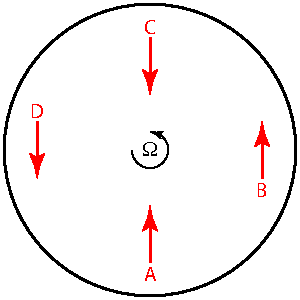
\includegraphics[width=\linewidth]{coriolis-exercise}
\caption[Movement on a merry-go-round]{Schematic for Exercise~\ref{ex:coriolis}.
\label{f.coriolis-exercise}}
\end{marginfigure}

\section{Lagrange and Roche}
For analyzing the motion of a test particle in the vicinity of two massive orbiting bodies, we transform to a frame with an origin at the center of mass mass and with an angular velocity $\Omega$.  The bodies have masses $M_{1}$ and $M_{2}$, and we take $M_{1}$ to be the more massive of the two bodies.  The two bodies are located at coordinates
\begin{eqnarray}
	M_{1}:&\qquad& x_{1} = -a\frac{M_{2}}{M},\,y_{1} = 0;\\
	M_{2}:&\qquad& x_{2} = a\frac{M_{1}}{M},\,y_{2} = 0,
\end{eqnarray}
Here $M = M_{1}+M_{2}$ is the total mass of the two bodies and $a$ their separation.

Let's check that our rotating coordinate system is consistent: since $M_{2}$ is at rest, the net force on it vanishes, so from equation~(\ref{e.motion-rotating}),
\[ -\frac{GM_{1}}{a^{2}} + a\frac{M_{1}}{M_{1}+M_{2}}\Omega^{2} = 0, \]
or
\[ P_{\mathrm{orb}}^{2} = \left(\frac{2\pi}{\Omega}\right)^{2} = \frac{4\pi^{2}}{GM}a^{3}. \]
This is just what we would expect from Kepler's law.

Now we are in a position to ask, are there any points where a particle could sit at rest in this frame?\marginnote{Remember, ``at rest in this frame'' means the particle is co-rotating with our two masses.}
Between the two masses, for example, we expect that the net force must vanish at some point. The acceleration of a test mass is 
\begin{equation}\label{e.test-mass-acceleration-x}
\DDtt{\rv} = -\frac{GM_{1}}{|\rv-\rv_{1}|^{3}}(\rv-\rv_{1}) - \frac{GM_{2}}{|\rv-\rv_{2}|^{3}}(\rv-\rv_{2}) + \frac{G(M_{1}+M_{2})}{a^{3}} \rv.
\end{equation}
Along the $x$-axis, points where a particle would feel no acceleration are given by the roots of the equations
\begin{eqnarray*}
	x < x_{1}:&\qquad& \frac{M_{1}}{(x_{1}-x)^{2}} + \frac{M_{2}}{(x_{2}-x)^{2}} + \frac{G(M_{1}+M_{2})}{a^{3}} x = 0;\\
	x_{1} < x < x_{2}:&\qquad& -\frac{M_{1}}{(x-x_{1})^{2}} + \frac{M_{2}}{(x_{2}-x)^{2}} + \frac{G(M_{1}+M_{2})}{a^{3}} x = 0;\\
	x_{2} < x:&\qquad& \frac{M_{1}}{(x-x_{1})^{2}} + \frac{M_{2}}{(x-x_{2})^{2}} + \frac{G(M_{1}+M_{2})}{a^{3}} x = 0.
\end{eqnarray*}
This is a nasty quintic equation; however, if we take the limit $M_{2}\ll M_{1}$ then after some inspired algebra we find that there are three roots, which are the first three \textbf{Lagrange points}:
\begin{eqnarray*}
L_{1}: &\qquad& x_{L1} \approx a\left\{\frac{M_{1}}{M_{1}+M_{2}} - \left[\frac{M_{2}}{3(M_{1}+M_{2})}\right]^{1/3}\right\};\\
L_{2}: &\qquad& x_{L2} \approx a\left\{\frac{M_{1}}{M_{1}+M_{2}} + \left[\frac{M_{2}}{3(M_{1}+M_{2})}\right]^{1/3}\right\};\\
L_{3}: &\qquad& x_{L3} \approx a\left\{-\frac{M_{1}+2M_{2}}{M_{1}+M_{2}} + \frac{7M_{2}}{12M_{1}}\right\}.
\end{eqnarray*}
These points are depicted in Fig.~\ref{f.Roche} for a system with $M_{2} = 0.05\,M_{1}$.
The remaining two Lagrange points $L_{4}$ and $L_{5}$ form equilateral triangles with $M_{1}$ and $M_{2}$.
\begin{marginfigure}
\includegraphics[width=\linewidth]{Roche}
\caption{Lagrange points for a system with $M_{2} = 0.1\,M_{1}$.
\label{f.Roche}}
\end{marginfigure}
We can draw an equipotential surface (in the rotating frame) that crosses through $L_{1}$: the surface is dumbbell-shaped and forms two \textbf{Roche lobes} (Fig.~\ref{f.Roche}) that touch at $L_{1}$.  Within each lobe the gradient of the potential is inward toward the center of the lobe.

\begin{exercisebox}[Vanishing acceleration at $L_{4}$]
Show that the acceleration vanishes at $L_{4}$:
\begin{enumerate}\renewcommand{\labelenumi}{\alph{enumi})}
   \item Find the coordinates of $L_{4}$;
   \item Compute the net gravitational acceleration, due to both $M_{1}$ and $M_{2}$, on a particle at point $L_{4}$ and show that it points toward the center of mass; then
   \item Show that the gravitational acceleration cancels the centrifugal, so that the net acceleration vanishes.
\end{enumerate}
\end{exercisebox}

\newthought{From the expressions for $L_{1}$ and $L_{2}$, we notice that} they can be written
as
\sidenote{Recall that
\[ a\frac{M_{1}}{M_{1}+M_{2}} = x_{2}, \]
the location of body 2.}
\[ 
	x_{L1} \approx x_{2} - R_{\mathrm{H}};\quad x_{L2}\approx x_{2} + R_{\mathrm{H}},
\]
with
\[ R_{\mathrm{H}}\approx a\left[\frac{M_{2}}{3(M_{1}+M_{2})}\right]^{1/3}. \]
Particles within a sphere of radius $R_{\mathrm{H}}$ are dominated by the gravitational attraction of $M_{2}$; $R_{\mathrm{H}}$ is called the \textbf{Hill radius}.

\begin{exercisebox}[Hill radius of the Sun-Jupiter system]
Compute the Hill radius for the Sun-Jupiter system.
\end{exercisebox}

\begin{exercisebox}[Overflow of Roche lobe]
Speculate on what would happen if $M_{2}$ had an atmosphere that extended outside its Roche lobe.
\end{exercisebox}

\section{Tidal forces}
Because a planet is extended, the gravitational force exerted by another mass on it varies across its diameter. As a warm-up, let's imagine putting four test masses some distance from the Earth and letting them free-fall.  We have a camera that is aligned with the center of mass of these four particles and that free-falls with them.
\begin{marginfigure}
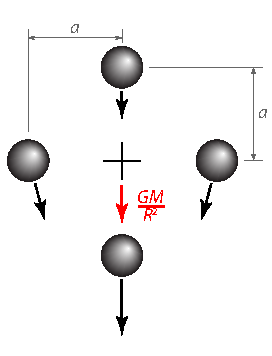
\includegraphics[width=\linewidth]{Tides}
\caption[Four freely falling bodies]{Four freely falling bodies.  In a frame that falls with them, how does their motion appear?
\label{f.tides}}
\end{marginfigure}

Figure~\ref{f.tides} depicts the setup: the particles are a distance $a$ from the center of mass (indicated with a cross) and the center of mass is a distance $R$ from the Earth's center.
When we release the particles and camera, the camera and center of mass both move downward with acceleration $-GM/R^{2}\bvec{\hat{z}}$.  Because each particle feels a slightly different gravitational force, however, none of the particles falls with that exact acceleration: the top particle has a lower acceleration and the bottom, higher; while the left and right particles have some horizontal acceleration 
toward the center of mass.

\begin{exercisebox}[Demonstration of tidal acceleration]
\label{ex:simple-tidal}
Compute the difference between the acceleration of each test mass and that of the center of mass.  Expand this difference to lowest order in $a/R$.  This difference is the \textbf{tidal force}.  Sketch the tidal force on each particle from the point of view of the free-falling camera.
\end{exercisebox}

\begin{figure*}[hbtp]
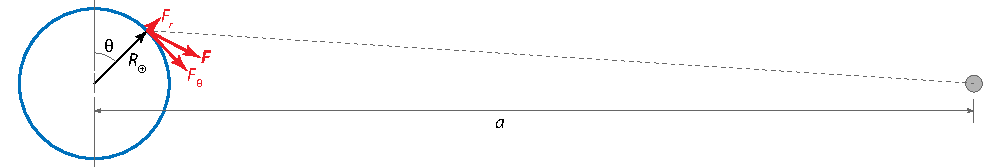
\includegraphics[width=\linewidth]{Earth-Moon-tides}
\caption[Tidal force on the Earth]{Schematic of the tidal force on the Earth raised by the Moon.
\label{f.Earth-Moon-tides}}
\end{figure*}

For the Earth-moon system (Fig.~\ref{f.Earth-Moon-tides}), we can decompose the tidal force exerted by the moon into radial and tangential components.  The Earth-Moon separation is $a = 60.3 R_{\Earth}$, so expanding our expression for the tidal force to lowest order in $R_{\Earth}/a$ is a good approximation.

Upon expanding\sidenote{The geometry can be worked out by consulting Fig.~\ref{f.Earth-Moon-tides}; it is straightforward, but tedious, and I won't go through the algebra here.} the tidal acceleration components to lowest order in $R_{\Earth}/a$ are found to be
\begin{eqnarray}
\label{e.moon-tide-radial}\rhat: &\qquad& \frac{GM_{\Moon}R_{\Earth}}{a^{3}}\left(3\sin^{2}\theta - 1\right)\\
\label{e.moon-tide-tangential}\thetahat: &\qquad& \frac{3GM_{\Moon}R_{\Earth}}{2a^{3}}\sin2\theta.
\end{eqnarray}
\begin{exercisebox}[Radial component of tidal force]
Sanity check: does the radial component of the tidal force, eq.~(\ref{e.moon-tide-radial}), agree with the calculation in Exercise~\ref{ex:simple-tidal}?
\end{exercisebox}
\begin{marginfigure}
\includegraphics[width=\linewidth]{lunar-tidal-force}
\caption[Components of the tidal force]{Tidal force field exerted by the Moon on the Earth.
\label{f.lunar-tidal-force}}
\end{marginfigure}
\noindent The ratio of the radial component of the tidal acceleration, neglecting the angular dependence, to the Earth's surface gravity is
\[ \frac{M_{\Moon}}{M_{\Earth}}\left(\frac{R_{\Earth}}{a}\right)^{3} = \sci{5.6}{-8}. \]
This is quite small, and you might wonder how the tidal force can produce such large daily flows of water in the ocean.  But consider the tangential component, eq.~(\ref{e.moon-tide-tangential}): it has a maximum at $\theta = 45^{\circ},\,135^{\circ}$ and, although it is also small, there is nothing to oppose it.

\newthought{The Earth's rotational period is shorter than the Moon's orbital period.} Because of viscosity (resistance to flow) the tidal bulge is carried ahead of the line joining the centers of the Earth and Moon (Figure~\ref{f.tidal-torque}).  As a result, the Moon's pull exerts a torque on the Earth and gradually slows its rotation; the oblate Earth in turn exerts a torque on the Moon and gradually forces it to greater orbital separation.

\begin{figure*}
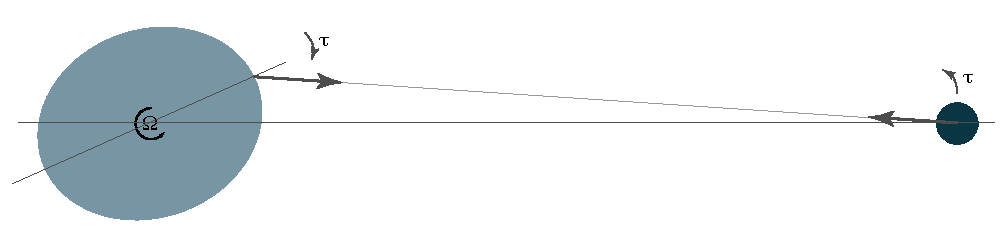
\includegraphics[width=\linewidth]{tidal-torque}
\caption[Torque on the Earth's tidal bulge]{The torque resulting from the misalignment of Earth's tidal bulge.
\label{f.tidal-torque}}
\end{figure*}

\section{Angular Momentum}\label{s.angular-momentum}
There is another way of looking at the spin-orbit interaction of the Earth and Moon.  What is the spin angular momentum of the Earth? What is the orbital angular momentum of the Moon and Earth? How do they compare?

The angular momentum of a particle of mass $m$ is
\begin{equation}\label{e.def-L}
	\bvec{L} = \bvec{r}\vcross m\bvec{v}.
\end{equation}
For a particle in a circular orbit, $\bvec{v} = r\Omega \thetahat$; using Kepler's law, we have
\[	L = mr^{2}\Omega = m\left(GMr\right)^{1/2}, \]
where $r$ is the distance from the center of mass.  The direction of $\bvec{L}$ is perpendicular to the plane of the orbit.  For two bodies orbiting a common center of mass, the problem is equivalent to a single particle of mass
\[ \mu = \frac{M_{1}M_{2}}{M_{1}+M_{2}} \]
orbiting a \emph{fixed} mass $M_{1}+M_{2}$ at a distance $a$, where $a$ is the separation of the two bodies.  Hence the orbital angular momentum of the two-body system is
\begin{equation}\label{orbital-2-two-body}
	L = \mu a^{2}\Omega = \frac{M_{1}M_{2}}{M_{1}+M_{2}}\left[G\left(M_{1}+M_{2}\right)a\right]^{1/2}.
\end{equation}
The orbital angular momentum increases with separation $a$.

\begin{marginfigure}
\includegraphics[width=\linewidth]{Inertia}
\caption{Calculation of the moment of inertia for a sphere. \label{f.inertia}}
\end{marginfigure}

Now for the spin angular momentum.  Let's take a simple case, that of a sphere of uniform density $\rho = 3M/(4\pi R^{3})$.  The sphere rotates uniformly with angular velocity $\Omega$.  To find the total angular momentum, we add up the contributions from infinitesimal bits.  To make this easy, we'll use the geometry shown in Figure~\ref{f.inertia}.  We'll divide our sphere into shells, each a distance $r$ from the center and of thickness $\dif r$.  Then we'll slice each shell into rings of width $r\,\dif\theta$.  We'll add up the angular momentum of the rings to find the angular momentum of shell, and then sum up the angular momentum of the shells to get the total.

%\begin{marginfigure}
%\includegraphics[width=\linewidth]{inertia-x-section}
%\caption{Cross-section of ring.\label{f.inertia-x-section}}
%\end{marginfigure}
Consider a cross-section of a ring.  The angular momentum is perpendicular to both $\bvec{r}$ and $\bvec{v}$; when we add up all of the pieces around the ring, the horizontal parts cancel, leaving the vertical part.  The mass of the ring is $\rho\times 2\pi r\sin\theta\,\dif r\,r\dif\theta$; the velocity is $r\sin\theta \times \Omega$.  The vertical component of the ring's angular momentum is therefore
\[
	\dif L_{\mathrm{ring}} = 2\pi \rho\Omega r^{4}\sin^{3}\theta\, \dif \theta \,\dif r.
\]
To get the angular momentum of a shell, we integrate over $\theta$:
\[
	\dif L_{\mathrm{shell}} = 2\pi\rho\Omega r^{4}\,\dif r\,\int_{0}^{\pi}\sin^{3}\theta\,\dif\theta.
\]
To do the integral, write $\sin^{3}\theta = (1-\cos^{2}\theta)\sin\theta$; then change variables to $\mu = \cos \theta$: in that case $\dif\mu = -\sin^\theta\,\dif\theta$, $\mu(\theta = 0) = 1$, and $\mu(\theta=\pi)=-1$.  The integral is then
\[
	\int_{0}^{\pi}\sin^{3}\theta\,\dif\theta = \int_{-1}^{1}(1-\mu^{2})\,\dif\mu 
		= \frac{4}{3},
\]
and the angular momentum of our shell is
\[
	\dif L_{\mathrm{shell}} = \frac{8\pi}{3}\rho\Omega r^{4}\,\dif r.
\]
Finally, integrate over $r$ to get the angular momentum of the sphere,
\begin{equation}\label{e.ang-momentum-sphere}
	L = \frac{8\pi}{3}\rho\Omega \int_{0}^{R}r^{4}\,\dif r = \frac{8\pi}{15}\rho\Omega R^{5} = \frac{2}{5} MR^{2}\Omega.
\end{equation}
In this last equation we substituted for $\rho = 3M/(4\pi R^{3})$. If the density is not uniform, but is higher toward the center, then the angular momentum is reduced. For example, the Earth's moment of inertia is $0.331 MR^{2}$ (see Table E.15 of \citetalt{Lissauer2013Fundamental-Pla}).

\begin{exercisebox}[Orbital angular momentum of the Earth-Moon system]
Compute the orbital angular momentum of the Earth-Moon system.  Compute the spin angular momentum of the Earth. Compare the two.
\end{exercisebox}

\begin{exercisebox}[Affect of central concentration on the moment of inertia]
Explain why having a higher density toward the center of a planet would reduce the moment of inertia.
\end{exercisebox}

% %!TEX root = ../AST208-notes.tex

\section{Warmup: the simple harmonic oscillator}

Let's begin with a simple system: a mass $m$ attached to a spring with force constant $k$. We'll neglect any dissipation (friction), and then add a driving oscillatory force. In reading these notes, don't dwell so much on the mathematical details; instead try to focus on the gross behavior of the solutions.

\subsection{With no driving force}

\begin{marginfigure}
\includegraphics[width=\linewidth]{simple-spring}
\caption[A simple harmonic oscillator]{A simple harmonic oscillator: a mass $m$ on a frictionless surface attached to a  spring with force $F = -kx$.
\label{f.simple-spring}}
\end{marginfigure}

If we put the origin of our coordinate system where the mass is at rest with the spring relaxed, then the equation of motion of the mass is
\begin{equation}\label{e.SHO-basic}
	\DDtt{x} + \frac{k}{m} x = 0.
\end{equation}
You have solved this before: the most general solution is
\begin{equation}\label{e.SHO-general-solution}
	x(t) = x_{0}\cos(\wot) + \frac{v_{0}}{\omega_{0}}\sin(\wot)
\end{equation}
with $\omega_{0}^{2} = k/m$ and with $x_{0}$ and $v_{0}$ being the initial position and velocity of the mass.

\begin{exercisebox}[Solutions to equations for a simple harmonic oscillator]
Verify that equation (\ref{e.SHO-general-solution}) is a solution to equation (\ref{e.SHO-basic}) with initial conditions $\left.x\right|_{t=0}=x_{0}$, $\left.\dif x/\dif t\right|_{t=0} = v_{0}$.
\end{exercisebox}

\subsection{With driving at frequency $\omega \neq \omega_{0}$}

Now let us push on our mass with an oscillating force, $F\cos(\omega t)$ with $\omega\neq\omega_{0}$. A real world example would be holding a vibrating tuning fork near one tuned to a different frequency.  The equation of motion is now
\begin{equation}\label{e.SHO-driven}
	\DDtt{x} + \omega_{0}^{2}x = \frac{F}{m}\cos(\wt).
\end{equation}
You can verify by substitution that a general solution is
\[
	x(t) = \frac{F/m}{(\omega_{0}^{2}-\omega^{2})}\cos(\wt) + A\cos(\wot)+B\sin(\wot).
\]
Let's start with our harmonic oscillator at rest ($v_{0} = \left.\dif x/\dif t\right|_{t=0} = 0$) and at $\left. x\right|_{t=0} = 0$.  With these conditions, we can determine the constants $A$ and $B$; the solution is
\[
	x(t) = \frac{F/m}{(\omega_{0}^{2}-\omega^{2})}\left[\cos(\wt)-\cos(\wot)\right].
\]
Let's recast this by defining $\Delta = \omega_{0} - \omega$, $\omega_{m} = (\omega_{0}+\omega)/2$.  Then
\begin{eqnarray*}
  \omega_{0}^{2}-\omega^{2} &=& (\omega_{0}-\omega)(\omega_{0}+\omega) = 2\Delta\omega_{m},\\
  \cos(\wot) &=& \cos\left(\wmt+\Delta t/2\right) = \cos(\wmt)\cos(\Delta t/2) - \sin(\wmt)\sin(\Delta t/2),\\
  \cos(\wt) &=& \cos\left(\wmt-\Delta t/2\right) = \cos(\wmt)\cos(\Delta t/2) + \sin(\wmt)\sin(\Delta t/2);
\end{eqnarray*}
and we write the solution as
\begin{equation}\label{e.beats}
	x(t) = \left[\frac{F/m}{\Delta\omega_{m}}\sin(\Delta t/2)\right]\sin(\wmt).
\end{equation}
This illustrates the phenomena of \textbf{beats}: the oscillation consists of a carrier signal at frequency $\omega_{m}$ with the amplitude modulated at the slower frequency $\Delta /2$.  Notice that the amplitude increases as $\Delta \to0$, i.e., $\omega\to\omega_{0}$.

\begin{figure*}[hbt]
\includegraphics[width=\linewidth]{beats}
\caption[Illustration of beats for four different frequencies]{Illustration of beats for four different frequencies $\omega$.  Notice how the amplitude increases as $\Delta$ becomes smaller.
\label{f.beats}}
\end{figure*}

\subsection{With driving at frequency $\omega_{0}$}

As we saw in the previous example, the amplitude of the driven oscillation increases as $\omega\to\omega_{0}$.  Now let's drive the oscillator precisely at its natural frequency $\omega_{0}$.  The equation of motion is
\begin{equation}\label{e.driven-at-resonance}
	\DDtt{x} + \omega_{0}^{2}x = \frac{F}{m}\cos(\omega_{0}t).
\end{equation}
The general solution is
\[
	x(t) = \frac{Ft}{2m\omega_{0}}\sin(\wot) + A\cos(\wot) + B\sin(\wot).
\]
Notice that the response to the driving grows linearly in time. Suppose our mass has been oscillating with no driving, and at $t=0$ we turn on $F$.  Suppose further that at time $t=0$ the position of the mass is $0$ and the velocity of the mass is $v_{0}$.  Then our solution is
\begin{equation}\label{e.resonant-oscillator}
	x(t) = \left[\frac{Ft}{2m\omega_{0}} + \frac{v_{0}}{\omega_{0}}\right]\sin(\wot).
\end{equation}

\begin{exercisebox}[Solutions to equations for a driven oscillator]
Verify that equation~(\ref{e.resonant-oscillator}) is a solution to equation~(\ref{e.driven-at-resonance}).  For the resonant oscillation in eq.~(\ref{e.resonant-oscillator}), what is the time for the amplitude to double?
\end{exercisebox}

\newthought{In reality, other effects may eventually limit the amplitude's growth.} The spring may snap when stretched too far. The wine glass may shatter when the singer hits a high note. Nevertheless, when a driving term oscillates near a natural frequency in the system, the result is for the oscillation amplitude to grow.
\section{The damped, driven oscillator}

For completeness, let's make our model even more realistic by adding some \textbf{damping}.  We add a friction or drag force that is proportional to velocity, $F_{\mathrm{friction}} = -\Gamma \dif x/\dif t$. Our complete equation of motion is then
\begin{equation}
	\DDtt{x} + \frac{\Gamma}{m} \DDt{x} + \omega_{0}^{2}x = \frac{F}{m}\cos(\omega t).
\end{equation}
The solution to this is more complicated than the previous examples, but it is found using the same technique.  The general solution for initial conditions $\left.x\right|_{t=0} = x_{0}$ and $\left.\dif x/\dif t\right|_{t=0} = v_{0}$ is
\begin{eqnarray}
\label{e.general-solution-ddo}
x(t) &=& \frac{F\womw/m}{\womw^{2}+\gw}\cos(\omega t) \\
	&& + \frac{\Gamma\omega F/m^{2}}{\womw^{2}+\gw}\sin(\omega t)\nonumber \\
	&& + \left[x_{0}-\frac{F\womw/m}{\womw^{2}+\gw}\right]e^{-\Gamma t/2m} \cos(\omega_{\Gamma}t) \nonumber\\
	&& + \left[\frac{v_{0}}{\omega_{\Gamma}}-\frac{\Gamma\omega F/m^{2}}{\womw^{2}+\gw}
	\,\frac{\omega}{\omega_{\Gamma}}\right]e^{-\Gamma t/2m} \sin(\omega_{\Gamma}t), 
	\nonumber
\end{eqnarray}
with
\[ \omega_{\Gamma} = \omega_{0}\left(1-\frac{(\Gamma/m)^{2}}{4\omega_{0}^{2}}\right)^{1/2}. \]
This formula is long, so let's look at limiting cases.  First, suppose we turn off the driving force by setting $F\to 0$. Also, let's set $v_{0}\to0$ as well. Then
\[
	x(t) = x_{0}e^{-\Gamma t/2m} \cos\left(\omega_{\Gamma}t\right).
\]
This is similar to our simple example, but the frequency is slightly shifted from $\omega_{0}$ to $\omega_{\Gamma}$,
and the amplitude decays as $e^{-\Gamma t/2m}$. A plot is shown in Figure~\ref{f.damped}.

\begin{figure*}[ht]
\includegraphics[width=\linewidth]{damped}
\caption[A damped oscillator]{A damped oscillator, with frequency $\omega_{0} = 2\pi$ and damping constant $\Gamma/m = 0.04\pi$. The light gray vertical lines indicate the period $2\pi/\omega_{0}$.
\label{f.damped}}
\end{figure*}

Now if we turn on our driving force $F$ and set $\Gamma\to0$, then we recover equation~(\ref{e.beats}), as expected. So, for the general case, we expect that the oscillation will look like that in Figure~\ref{f.beats} at early times. After a time $2m/\Gamma$, however, the last two terms of equation (\ref{e.general-solution-ddo}) will decay and there will only be the first two terms, which oscillate at frequency $\omega$.  Figure~\ref{f.damped-driven} shows the solution in this case.  The light gray vertical lines mark off periods $2\pi/\omega_{0}$; you can see that as the beats disappear the frequency shifts from approximately $\omega_{0}$ to $\omega$.

\begin{figure*}[ht]
\includegraphics[width=\linewidth]{damped-driven}
\caption[A damped, driven oscillator]{A damped, driven oscillator, with frequency $\omega_{0} = 2\pi$, damping constant $\Gamma/m = 0.04\pi$, and driving force $4.0/m\,\cos(\omega t)$ with $\omega=1.7\pi$. The light gray vertical lines indicate the period $2\pi/\omega_{0}$.
\label{f.damped-driven}}
\end{figure*}

In the limit $\omega \to \omega_{0}$ the solution goes to 
\[ x(t) = \frac{F}{\Gamma\omega_{0}} \sin(\omega_{0} t).\]
For the parameters used to make Figure~\ref{f.damped-driven}, this amplitude is $F/(\Gamma\omega_{0}) = 5.1$; the final oscillation amplitude for the case shown in the plot is much less than this because the driving frequency is $\omega = 0.85\omega_{0}$.

\section{Applications to the solar system}
Planets, moons, and other minor bodies in solar system have made millions to billions of orbits. As the previous section demonstrates, even a small perturbing force, if applied near a natural frequency of a system, can eventually produce a large response when applied over such a long dynamical time. 

There are many bodies in the solar system that are locked into a stable resonance. For example, Pluto is locked into a stable 2:3 resonance with Neptune (that is, Pluto completes 2 orbits for every 3 of Neptune), and the Jovian moons Io, Europa, and Ganymede are locked into a 1:2:4 resonance. Resonances can also lead to instability, in which a body's orbit is distorted to the point that it crosses the orbit of another planet, at which point that body either collides with the other planet or is scattered out of the solar system.  For example, the Kirkwood gap in the asteroid belt is located at the 3:1 resonance with Jupiter (see Fig.~2.10 of \citetalt{Lissauer2013Fundamental-Pla}). Numerical calculations find that the precession of Mercury's perihelion is coming into resonance with that of Jupiter, leading to a 1\% chance over the next \val{5}{\Giga\yr} of Mercury colliding with the Sun or Venus, and a smaller possibility of the entire inner solar system becoming unstable\cite{Laskar2009Existence-of-co} over that time.

\newthought{Torques exerted on a planet's equatorial bulge} by other solar system bodies can cause that planet's obliquity to vary.  Saturn's large (relative to Jupiter) axial tilt is thought to be caused by a spin-orbit resonance between the precession of Saturn's axis the precession of Neptune's orbital plane\cite{Ward2004Tilting-Saturn.}.  Mars's axial tilt wanders considerably over a few Myr timescale and has reached tilts as large as $60^{\circ}$ in the past.  The large moment of inertia of the Earth-Moon system keeps Earth's axial tilt from wandering to such extreme values; nevertheless, the Earth's inclination does oscillate by $<1^{\circ}$ on a $\val{40\,000}{\yr}$ timescale.  This wandering of the inclination, along with variations in the orbital eccentricity, are thought to explain the quasi-periodic ice ages on Earth over the last few million years\cite{Zachos2001Trends-Rhythms-}.


% %!TEX root = ../AST208-notes.tex

\begin{quote} It's more important to know whether there will be weather than what the weather will be. ---Norton Juster, \emph{The Phantom Tollbooth}\end{quote}

\section{Hydrostatic equilibrium}

Let's consider a fluid at rest in a gravitational field. By \emph{at rest}, we simply mean that the fluid velocity is sufficiently small that we can neglect the inertia of the moving fluid in our equation for force balance.  By a \emph{fluid}, we mean that the pressure is isotropic\sidenote{Meaning the pressure is the same in all directions.} and directed perpendicular to a surface.  Let's now imagine a small fluid element, with thickness $\Delta r$ and cross-sectional area $\Delta A$, as depicted in Fig.~\ref{f.hydrostatic-equilibrium}.
\begin{marginfigure}
\includegraphics[width=\linewidth]{hydrostatic-equilibrium}
\caption[A fluid element in hydrostatic equilibrium]{A fluid element in hydrostatic equilibrium.
\label{f.hydrostatic-equilibrium}}
\end{marginfigure}

The weight of the fluid element is $\Delta m g$, where $g$ is the gravitational acceleration and $\Delta m =  \Delta A\times\Delta r\times \rho$ is the mass of the fluid element with $\rho$ being the mass density.
The force on the upper face is $\Delta A\times P(r+\Delta r)$; on the lower face, $\Delta A\times P(r)$.  Here $P(r)$ is the pressure.  For the element to be in hydrostatic equilibrium the forces must balance,
\[
	\Delta A \left[ -P(r+\Delta r) + P(r) - \Delta r \rho g  \right] = 0;
\]
dividing by $\Delta r$ and taking the limit $\Delta r \to 0$ gives us the equation of hydrostatic equilibrium:
\begin{equation}\label{e.hydrostatic-equilibrium}
	\DD{P}{r} = -\rho g.
\end{equation}
For an incompressible fluid in constant gravity, the pressure increases linearly with depth. This is a good approximation to the pressure in Earth's oceans.  In general, however, the density $\rho$ depends on the pressure $P$, and we need more information to solve for the atmospheric structure.

\marginnote{The SI unit of pressure is the \textbf{Pascal}: $\val{1}{\unitstyle{Pa}} = \val{1}{\unitstyle{N}\usk\meter^{-2}}$. The mean pressure at terrestrial sea level is $\val{1}{\unitstyle{atm}} = \val{\sci{1.013}{5}}{\unitstyle{Pa}}$. Other common units of pressure are the \textbf{bar} ($\val{1}{\unitstyle{bar}} = \val{10^{5}}{\unitstyle{Pa}}$) and the \textbf{Torr} ($\val{760}{\unitstyle{Torr}} = \val{1}{\unitstyle{atm}}$).}
\begin{exercisebox}[Pressure increase in water]
Water is nearly incompressible and has a density of $\val{10^{3}}{\kilo\gram\usk\meter^{-3}}$.  How deep would you need to dive for the pressure to increase by $\val{1}{\unitstyle{atm}} = \val{\sci{1.013}{5}}{\unitstyle{Pa}}$?  The gravitational acceleration at Earth's surface is $\val{9.8}{\meter\usk\second^{-2}}$.
\end{exercisebox}

Let's look at this in a bit more detail.  Suppose we take our fluid layer to be thin, so that $g$ is approximately constant. Then we can write equation~(\ref{e.hydrostatic-equilibrium}) as
\[ \int_{P_{0}}^{P_(z)} \dif P = -g\int_{0}^{z} \rho\,\dif z. \]
Now consider a cylinder of cross-section $\Delta A$ that extends from $0$ to $z$.  The mass of that cylinder is
\[ m(z) = \Delta A\times\int_{0}^{z}\rho \,\dif z.
\]
and its weight is $m(z)g$.
\begin{marginfigure}
\centering\includegraphics[width=0.8\linewidth]{column}
\caption[The mass of a column of fluid]{
The mass of a column of fluid.
\label{f.column}}
\end{marginfigure}

The difference in pressure between the bottom and top of the cylinder is just
\[ P_{0}-P(z) = g m(z)/\Delta A, \]
that is, the weight per unit area of our column.  Let's apply this to our atmosphere:
if we take the top of our column to infinity and the pressure at the top to zero, then the pressure at the bottom (sea level) is just the weight of a column of atmosphere with a cross-sectional area of $\val{1}{\meter^{2}}$.

\section{The ideal gas}\label{s.ideal-gas}
To solve equation~(\ref{e.hydrostatic-equilibrium}) we need at a minimum a relation between pressure and density. A relation between pressure, density, and temperature is called an \textbf{equation of state}.
For an ideal gas\sidenote[][\baselineskip]{By \emph{ideal} gas, we mean that the particles are non-interacting; as a result, the energy of the gas only depends on the kinetic energy of the particles and in particular is independent of the volume.} of $N$ particles in a volume $V$ at pressure and temperature $P$ and $T$, the equation of state is
\begin{equation}\label{e.ideal-gas-eos}
PV = NkT
\end{equation}
where $k = \val{\sci{1.381}{-23}}{\unitstyle{J}\usk\K^{-1}}$ is \textbf{Boltzmann's constant}.

In chemistry, it is convenient to count the number of particles by \textbf{moles}.  One mole of a gas has $\NA = \sci{6.022}{23}$ particles\sidenote{The constant $\NA$ is known as \textbf{Avogadro's number}.}, and the number of moles in a sample is $n = N/\NA$.  If we divide and multiply equation~(\ref{e.ideal-gas-eos}) by $\NA$, then our ideal gas equation becomes
\[ PV = n\left[\NA k\right]T \equiv n R T, \]
where $R = \NA k = \val{8.314}{\unitstyle{J}\usk\K^{-1}\usk\mol^{-1}}$ is the gas constant. This is perhaps the most familiar form of the ideal gas law---but it is not in a form useful to astronomers.

We astronomers don't care about little beakers of fluid---we have whole worlds to model! Let's take our ideal gas law and introduce the molar weight $m$ as the mass of one mole of our gas.  Then the ideal gas law can be written
\begin{equation}\label{e.ideal-gas-astro}
 P = \left(\frac{mN/\NA}{V}\right)\frac{k\NA}{m} T \equiv \rho \frac{k\NA}{m} T.
\end{equation}
The quantity in parenthesis is the mass per volume, or density $\rho$, of our fluid.  This is the same mass density that appears in equation~(\ref{e.hydrostatic-equilibrium}).  Equation~(\ref{e.ideal-gas-astro}) is the form most convenient for fluid dynamics, because it is in terms of intrinsic fluid properties rather than in terms of a laboratory quantity like volume.

\section{The scale height}\label{s.scale-height}
Let's take a first stab at modeling Earth's atmosphere with equation~(\ref{e.hydrostatic-equilibrium}). We'll take Earth's atmosphere to be an ideal gas and for simplicity we'll assume the temperature doesn't change with altitude\sidenote[][-\baselineskip]{This isn't true, of course, but let's keep things simple and see how we do.}  The molar weight of dry\sidenote[][\baselineskip]{The water vapor content of air varies considerably depending on ambient conditions.} air is $\val{0.02897}{\kilo\gram\usk\mol^{-1}}$.  Using equation~(\ref{e.ideal-gas-astro}) to eliminate $\rho$ in equation~(\ref{e.hydrostatic-equilibrium}), we obtain
\[
	\frac{1}{P}\DD{P}{z} = -\frac{mg}{\NA kT},\quad\textrm{or} \quad\frac{\dif P}{P} = -\frac{mg}{\NA kT}\,\dif z.
\]
Integrating from $z=0$, where $P(z=0)=P_{0}$, to a height $z$ gives us an equation for the pressure as a function of height,
\begin{equation}\label{e.exp-atm}
	P(z) = P_{0}\exp\left[-\frac{mgz}{\NA kT}\right].
\end{equation}
Since the argument of the exponential is dimensionless, we see that we can write $P(z) = P_{0}e^{-z/H_{P}}$, where
\[  H_{P} = \frac{\NA kT}{mg} \]
is the \textbf{pressure scale height}---the height over which the pressure decreases by a factor $1/e$.

\begin{exercisebox}[Scale height for dry air]
Evaluate $H_{P}$ for dry air at a temperature of $\val{288}{\K}$ ($\val{15}{^{\circ}\unitstyle{C}}$).  Check that your answer is reasonable based on your experience.  In fact, this value of $H_{P}$ is overly large because the temperature in the troposphere does, in fact, decrease with height at an average \textbf{lapse rate} of
\[
	\DD{T}{z} = -\val{6.5}{^{\circ}\unitstyle{C}\usk\kilo\meter^{-1}}.
\]
\end{exercisebox}

\section{The adiabatic thermal gradient}\label{s.adiabatic-gradient}
Hot air rises. This simple phenomenon sets the lapse rate in the troposphere. Warm surface air rises quickly enough that there is little exchange of heat with colder, downward moving air.  As a result, the fluid motions are \textbf{adiabatic}.  To understand what this means, recall the first law of thermodynamics\cite{Fermi1956Thermodynamics}, which relates the change in internal energy $\dif U$ and in volume $\dif V$ to the heat transferred $\dif Q$:
\begin{equation}\label{e.first-law-thermo}
	\dif Q = \dif U + P\dif V,
\end{equation}
where $P$ is the pressure.  Now, we aren't using volume to describe our fluid\sidenote{cf.\ eq.~(\ref{e.ideal-gas-astro})} so let's apply this equation to $\val{1}{\mol}$ of our fluid, and divide both sides by the molar mass $m$.  Then $Q$ refers to the heat transferred \emph{per kilogram}, and $U$ refers to the internal energy \emph{per kilogram}.  Instead of $\dif V$, we then have $\dif V/(\val{1}{\mol}\times m) = \dif(1/\rho) = -\rho^{-2}\dif\rho$.  Our first law, rewritten in terms of mass-specific quantities, is thus
\begin{equation}\label{e.first-law-thermo-astro}
	\dif Q = \dif U -\frac{P}{\rho^{2}}\dif \rho.
\end{equation}
Suppose we wish to express quantities in terms of temperature $T$ and density $\rho$: then
\[ \dif U = \tderiv{U}{T}{\rho}\dif T + \tderiv{U}{\rho}{T}\dif \rho, \]
and
\[ \dif Q = \tderiv{U}{T}{\rho}\dif T + \left[\tderiv{U}{\rho}{T} - \frac{P}{\rho^{2}}\right]\dif \rho. \]
Hence the heat needed to raise the temperature of one kilogram of fluid when holding density fixed is
\begin{equation}\label{e.CV}
C_{\rho} \equiv \tderiv{Q}{T}{\rho} = \tderiv{U}{T}{\rho}.
\end{equation}
For an ideal gas, $U = U(T)$ and $C_{\rho}$ is approximately constant; hence we may integrate equation~(\ref{e.CV}) to obtain $U = C_{\rho}T + \textrm{const.}$.

In Eq.~(\ref{e.first-law-thermo-astro}), the last term is $-(P/\rho)\, \dif\rho/\rho = -(P/\rho)\,\dif\ln\rho$. This illustrates a useful trick: take the logarithm of the equation of state, $\ln (P) = \ln(\rho) + \ln (T) + \ln (k\NA/m)$, and then take the differential to obtain
\[ \frac{\dif P}{P} = \frac{\dif\rho}{\rho} + \frac{\dif T}{T}. \]
Now eliminate $\dif\rho/\rho$ in the equation
\[ \dif Q = C_{\rho}\dif T - \frac{P}{\rho}\frac{\dif\rho}{\rho} \]
to obtain an expression for the heat transferred as a function of temperature and pressure,
\[ \dif Q = \left[C_{\rho} + \frac{P}{\rho T}\right]\dif T - \frac{1}{\rho}\dif P
	 = \left[C_{\rho} + \frac{k\NA}{m}\right]\dif T - \frac{1}{\rho}\dif P. \]
From this we see that the heat needed to raise the temperature of one mole when holding pressure fixed is
\begin{equation}\label{e.CP}
C_{P}\equiv \tderiv{Q}{T}{P} = C_{V} + \frac{k\NA}{m}.
\end{equation}
The specific heat of one mole of various ideal gases is given in Table~\ref{t.specific-heat}.
\begin{table}
\caption{Specific heats for ideal gases.\label{t.specific-heat}}
\begin{tabular}{lrrr}
gas & $C_{\rho}$ & $C_{P}=C_{\rho}+k\NA/m$ & $\gamma = C_{P}/C_{\rho}$\\
\hline
monatomic & $(3/2) k\NA/m$ & $(5/2)k\NA/m$ & $5/3$\\
diatomic & $(5/2) k\NA/m$ & $(7/2)k\NA/m$ & $7/5$\\
\end{tabular}
\end{table}
It is important to remember that these relations for the specific heats are for an ideal gas and are not universally true.

\newthought{During convection, hot air rises and cool air descends, and both move adiabatically.}  By adiabatically, we mean that there is no heat exchange:
\[ 0 = \dif Q = C_{P}\dif T - \frac{1}{\rho} \dif P.\]
Using the ideal gas equation of state we can eliminate $\frac{1}{\rho} = (k\NA/m) T/P$ and write
\[ \frac{\dif T}{T} = \frac{k\NA}{mC_{P}} \frac{\dif P}{P} = \frac{C_{P}-C_{V}}{C_{P}} \frac{\dif P}{P} = \frac{\gamma-1}{\gamma}\frac{\dif P}{P}. \]
Integrating both sides of the equation gives
\[ \ln T = \frac{\gamma-1}{\gamma}\ln P + \textrm{const.},\]
or 
\begin{equation}\label{e.adiabat}
 T = T_{0}\left(\frac{P}{P_{0}}\right)^{(\gamma-1)/\gamma},
\end{equation}
where $T_{0}$ and $P_{0}$ are the temperature and pressure at the beginning of the adiabatic process.
Equation~(\ref{e.adiabat}) tells us how the temperature changes with pressure along an adiabat for an ideal gas.

\begin{exercisebox}[Adiabatic lapse rate]
Use equations~(\ref{e.adiabat}) and (\ref{e.hydrostatic-equilibrium}) to compute the lapse rate $\dif T/\dif z$ at sea level.  Dry air is composed of mostly diatomic gases with a molar weight $\val{0.02897}{\kilo\gram\usk\mol^{-1}}$. You should find an answer around $\val{-10}{^{\circ}\unitstyle{C}/\kilo\meter}$, which is almost twice as large as the value quoted earlier.  Can you guess why the value you calculated might be off? (\emph{Hint: there is a process we haven't yet accounted for.  If you want a hint, go outside and look up.})
\end{exercisebox}

\section{Atmospheric circulation on a rotating Earth}\label{s.motion-in-atmosphere}

The Sun heats the Earth unevenly; this in turn creates pressure gradients that drive a circulation of the atmosphere and a transfer for heat from the equator polewards.  The Coriolis force deflects the horizontal motion of the air, and this sets up large-scale features in the atmosphere.

Because of the Earth's rotation, in the frame of a particular location on Earth there is both a Coriolis and a centrifugal acceleration:
\begin{eqnarray}
\textrm{Coriolis} &\quad& \bvec{a}_{\mathrm{Cor}} = -2\bvec{\Omega}\vcross\bvec{v}\\
\textrm{centrifugal} &\quad& \bvec{a}_{\mathrm{cen}} = -\bvec{\Omega}\vcross\left(\bvec{\Omega}\vcross\bvec{R}\right)
\end{eqnarray}
where $\bvec{R}$ is the location of our particle and $\bvec{\Omega}$ is the rotation vector of the Earth.  

The centrifugal component just depends on the latitude $\lambda$ and causes the Earth to bulge at the equator to compensate. It doesn't, however, change the motion of air currents.  The vertical component of the Coriolis acceleration will be quite small compared to $\bvec{g}$, so we can neglect it as well. For the horizontal component, if we are at latitude $\lambda$,
\begin{marginfigure}
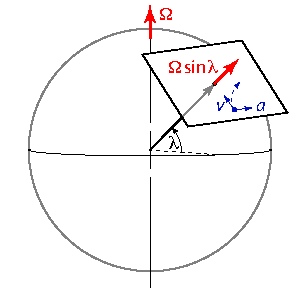
\includegraphics[width=\linewidth]{beta-plane}
\caption{Motion in a horizontal layer in a small region at latitude $\lambda$.}
\end{marginfigure}
\[
a_{\mathrm{Cor}} =  2\Omega v \sin\lambda.
\]
This acceleration is to the right in the northern hemisphere and to the left in the southern.  At the equator it vanishes.

\begin{exercisebox}[Coriolis vs.\ centripetal acceleration around a river bend]
Suppose we have a river flowing at $\val{3}{\kilo\meter/\hour}$.  At our latitude, how does the Coriolis acceleration compare to the centripetal acceleration if the river has a bend with radius of curvature $r$?  How large would $r$ need to be for the Coriolis force to dominate?
\end{exercisebox}

In addition to the Coriolis acceleration from the Earth rotation, horizontal pressure gradients will also produce an acceleration
\[
	-\frac{1}{\rho}\grad P.
\]
A typical horizontal gradient for a weather system is about $\val{0.03}{\milli\unitstyle{bar}/\kilo\meter}$.\marginnote{Recall that $\val{1}{\unitstyle{bar}} = \val{\sci{1.013}{5}}{\unitstyle{Pa}}$.  The density of air at sea level is $\val{1.3}{\kilo\gram\usk\meter^{-3}}$.} Consider a \textbf{cyclone} in which the winds swirl counterclockwise about a low.  Let's look at a small parcel of fluid a distance $r$ from the center of the cyclone, which has a height $H$. The mass of our fluid parcel is $\Delta S\,\Delta r\,H\,\rho$, and the acceleration of the fluid is $-v^{2}/r\,\hat{r}$. The equation for force and acceleration along $\hat{r}$ is therefore
\begin{marginfigure}
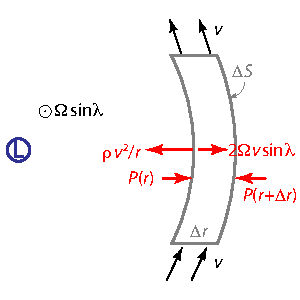
\includegraphics[width=\linewidth]{cyclone}
\caption{Forces on a parcel of air circulating about a low.
\label{f.cyclone}}
\end{marginfigure}
\[
	\left[P(r)-P(r+\Delta r)\right]\Delta S\,H + 2\Delta S\,\Delta r\,H\,\rho\,\Omega v\sin\lambda = -\Delta S\,\Delta r\,H\,\rho \frac{v^{2}}{r}.
\]
or
\begin{equation}\label{e.force-balance}
	\underbrace{\frac{v^{2}}{r}}_{\textrm{centripetal}} 
	+ \underbrace{2 v\Omega\sin\lambda}_{\mathrm{Coriolis}} 
	- \underbrace{\frac{1}{\rho}\DD{P}{r}}_{\mathrm{pressure}} = 0.
\end{equation}

\begin{exercisebox}[Scale of mid-latitude weather systems]
\begin{enumerate}
\renewcommand{\theenumi}{\alph{enumi}}
\renewcommand{\labelenumi}{\alph{enumi})}
\item\label{v-wind}
When $r$ is sufficiently large, we can neglect the centripetal term in equation~(\ref{e.force-balance}).  In that case, for a pressure gradient of $\val{3}{\milli\unitstyle{bar}}/\val{100}{\kilo\meter}$, what is a velocity satisfying this equation. Does this seem realistic?

\item Using the velocity you found in part \ref{v-wind}, determine the size $r$ of the weather system at which the centripetal term becomes comparable to the Coriolis term.
\end{enumerate}
\end{exercisebox}

In tropical regions the latent heat released from condensing water vapor in rising updrafts can produce a strong pressure gradient around a low---a tropical depression. If the pressure gradient is strong enough, a hurricane forms. In this case the pressure gradient can be as strong as $\val{0.3}{\milli\unitstyle{bar}/\kilo\meter}$, and the centripetal term cannot be neglected.
If we consider a hurricane located at  latitude $\lambda=20^{\circ}$ and take the eye region to have $r = \val{100}{\kilo\meter}$, then solving equation~(\ref{e.force-balance}) gives
\[
	v = -r\Omega\sin\lambda + \sqrt{(r\Omega\sin\lambda)^{2}+\frac{r}{\rho}\DD{P}{r}}\approx \val{46}{\meter/\second},
\]
which is typical of hurricane-strength winds.

\begin{exercisebox}[Why the strongest storms are associated with low-pressure systems]
You may have wondered why the strongest storms are associated with low-pressure systems. Repeat the analysis leading to equation~(\ref{e.force-balance}) for air circulating in an anti-cyclone around a pressure high. There is one crucial difference in the equation which leads to a limitation on the pressure gradient and velocities in this case; explain this difference.
\end{exercisebox}

% %!TEX root = ../planets-notes.tex

\section{Selected constants}
\begin{tabular}{lcrl}
\hline
constant & symbol & \multicolumn{2}{c}{value in MKS}\\
\hline\hline
speed of light & $c$ & $\sci{2.998}{8}$ & $\meter\usk\second^{-1}$\\
Newton constant & $G$ & $6.674\ee{-11}$ & $\meter^{3}\usk\kilo\gram^{-1}\usk\second^{-2}$ \\
Planck constant & $h$ & $6.626\ee{-34}$ & $\joule\usk\second$ \\ 
Planck constant, reduced & $\hbar$ & $1.055\ee{-34}$ & $\joule\usk\second$ \\
Boltzmann constant & $k$ & $1.381\ee{-23}$ & $\joule\usk\K^{-1}$ \\
Stefan-Boltzmann constant & $\sigma$ & $5.670\ee{-8}$ & $\watt\usk\meter^{-2}\usk\K^{-4}$ \\
 & $a = 4\sigma/c$ & $7.566\ee{-16}$ & $\joule\usk\meter^{-3}\usk\K^{-4}$ \\
mass, hydrogen atom & $m_{\mathrm{H}}$ & $1.673\ee{-27}$ & $\kilo\gram$ \\
atomic mass unit & $\mb$ & $1.661\ee{-27}$ & $\kilo\gram$\\
electron mass & $m_{e}$ & 9.109\ee{-31} & $\kilo\gram$\\
electron volt & $\eV$ & $1.602\ee{-19}$ & $\joule$ \\
\hline
\multicolumn{4}{c}{Astronomical}\\
\hline
solar mass & \Msun & $1.989\ee{30}$ & $\kilo\gram$ \\
solar radius & \Rsun & $6.960\ee{8}$ & $\meter$ \\
solar luminosity & \Lsun & $3.842\ee{26}$ & $\watt$ \\
solar effective temperature & $T_{\!\mathrm{eff,\odot}}$ & $5780$ & $\K$ \\
astronomical unit & AU & $1.496\ee{11}$ & $\meter$ \\
parsec & pc & $3.086\ee{16}$ & $\meter$ \\
year & yr & $3.154\ee{7}$ & $\second$ \\
\hline
\end{tabular}

\section{Properties of selected stellar types}
\begin{tabular}{crrrrr}
\hline
Spectral Type & $\Teff$ ($\K$) & $M/\Msun$ & $L/\Lsun$ & $R/\Rsun$ & $V$ mag.\\
\hline\hline
B5 & $15\,400$ & 5.9 & $830$ & 3.9 & -1.2\\
G0 & $5\,940$ & 1.05 & 1.4 & 1.1 & 4.4 \\
M5 & $3\,170$ & 0.21 & 0.0066 & 0.27 & 12.3\\
\hline
\end{tabular}

\section{Planets of the solar system}
\begin{tabular}{lcrrrr@{.}l}
\hline
Planet\rule{0pt}{2.5ex} & symbol & $a$ (AU) & $M$ ($\val{10^{24}}{\kilo\gram}$) & $R$ (km) & \multicolumn{2}{r}{$I/(MR^{2})$} \\
\hline\hline
Mercury & \mercury & 0.387 & 0.330 & 2\,440 & 0&353\\
Venus & \venus & 0.723 & 4.869 & 6\,052 & 0&33\\
Earth & \earth & 1.000 & 5.974 & 6\,371 & 0&331 \\
Mars & \mars & 1.524 & 0.642 & 3\,390 & 0&365\\
Jupiter & \jupiter & 5.203 & 1900 & 69\,900 & 0&254 \\
Saturn & \saturn & 9.543 & 569 & 58\,200 & 0&210\\
Uranus & \uranus & 19.192 & 86.8 & 35\,400 & 0&23\\
Neptune & \neptune & 30.069 & 102 & 24\,600 & 0&23\\
\hline
\end{tabular}


% %!TEX root = ../AST208-notes.tex

%!TEX root = ../planets-notes.tex
\section{A Brief Refresher on Trigonometry}

\subsection{Definitions in terms of the unit circle}

You may remember that in high school you memorized the definitions of the sine, cosine, and tangent of an angle in a right triangle.  The $\sin x$ is the ratio of the side of the triangle opposite the angle $x$ to the hypotenuse; the $\cos x$ is the ratio of the side adjacent the angle $x$ to the hypotenuse; and the $\tan x$ is the ratio of the side opposite the angle $x$ to the side adjacent the angle $x$. A useful mnemonic is \allcaps{soh-cah-toa}: Sine-Opposite-Hypotenuse --- Cosine-Adjacent-Hypotenuse --- Tangent-Opposite-Adjacent.

\begin{marginfigure}
\includegraphics[width=\linewidth]{high-school-triangle}
\label{f.high-school-triangle}
\end{marginfigure}

\newthought{You may have wondered why the tangent}, for instance, is called by that name.  Now that you are a  collegiate sophisticate, we can delve more deeply into how the sine, cosine, tangent, cotangent, secant, and cosecant are constructed.
Draw a circle with a radius of unit length.  Now draw a line from the origin $O$ to intersect the circle at a point $A$, as shown in Fig.~\ref{f.trig-schematic}.  Denote by $x$ the length along the arc from the horizontal to point $A$.

From the point $A$, we draw a vertical line to the horizontal.  The length of this line $AB$ is $\sin x$. Likewise, we draw a horizontal line from point $A$ to the vertical; the length of this line, which is equal to $OB$, we call $\cos x$.  

Next, we construct a line tangent to the arc at point $A$ and extend this \emph{tangent} to where it intersects the horizontal axis, at point $C$, and to where it intersects the vertical axis, at point $D$.  We call the length of the line $AC$ $\tan x$; the length of the line $AD$ we call $\cot x$.

\begin{marginfigure}[-6\baselineskip]
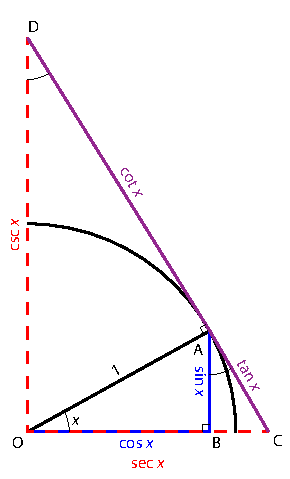
\includegraphics[width=\linewidth]{trig-schematic}
\caption[Construction from the unit circle]{Construction of the sine, tangent, secant, cosine, cotangent, and cosecant from the unit circle.}
\label{f.trig-schematic}
\end{marginfigure}

Finally, we draw from the origin $O$ lines along the horizontal to intersect the tangent at point $C$ and along the vertical to interest the cotangent at point $D$.  
The line from the origin $O$ to point $C$ is the \emph{secant} and we call the length $OC$ $\sec x$. The line $OD$ is the \emph{cosecant} and its length is $\csc x$.

The relationships between these quantities can be deduced by studying Fig.~\ref{f.trig-schematic}.  First, the triangle $ABC$ is similar to the triangle $OBA$. The ratio of $AC$ to $AB$ is therefore equal to the ratio of $OA$ to $OB$,
\begin{equation}\label{e.tan}
	\frac{AC}{AB} = \frac{\tan x}{\sin x} = \frac{OA}{OB} = \frac{1}{\cos x},\quad\textrm{so}
	\;\tan x = \frac{\sin x}{\cos x}.
\end{equation}
Likewise, the triangle $OAC$ is similar to $OBA$; therefore
\begin{equation}\label{e.sec}
	\frac{OC}{OA} = \frac{\sec x}{1} = \frac{OA}{OB} = \frac{1}{\cos x},\quad\textrm{so}
	\;\sec x = \frac{1}{\cos x}.
\end{equation}
Finally, the triangle $DAO$ is similar to $OBA$, giving
\begin{eqnarray}
	\frac{DO} {AO} = \frac{\csc x}{1} = \frac{OA}{BA} = \frac{1}{\sin x},&\quad&\textrm{so}
	\;\csc x = \frac{1}{\sin x},\label{e.csc}\\
	\frac{DA}{OA} = \frac{\cot x}{1} =  \frac{OB}{BA} = \frac{\cos x}{\sin x},&\quad&\textrm{so}
	\cot x = \frac{\cos x}{\sin x} = \frac{1}{\tan x}.\label{e.cot}
\end{eqnarray}
Some further relations follow immediately from the Pythagorean theorem:
\begin{eqnarray*}
	\sin^{2} x + \cos^{2} x &=& 1 \\
	\tan^{2} x + 1 &=& \sec^{2} x \\
	\cot^{x} x + 1 &=& \csc^{2} x.
\end{eqnarray*}
At small angles $x$, we see from the diagram that
$ \sin x < x < \tan x$, and $\cos x < 1$.
Further, one can show\cite{Courant1996What-is-Mathema} that
\begin{eqnarray}
	\lim_{h\to 0}\frac{\sin h}{h} = 1\quad\textrm{and}\label{e.lim-sine}\\
	\lim_{h\to 0}\frac{\cos h -1}{h} = 0.\label{e.lim-cosine}
\end{eqnarray}

\subsection{Trigonometric addition formulae}

To develop the formulae for $\sin(x+y)$ and $\cos(x+y)$, consider the schematic in Figure~\ref{f.trig-addition}. The grey arc is again a segment of a unit circle. The length of $OF$ is $\cos(x+y)$ and the length of $CF$ is $\sin(x+y)$.  By construction, $CE = \sin y$ and $OE = \cos y$.

\begin{marginfigure}
\includegraphics[width=\linewidth]{trig-addition}
\caption[Schematic of the addition of two angles]{Schematic of the addition of two angles $x$ and $y$.}
\label{f.trig-addition}
\end{marginfigure}

The length $CF = \sin(x+y)$ is the sum of $DF = EG$ and $CD$.  Now triangle $CDE$ is similar to $OBA$; hence
\[ 
	\frac{CD}{CE} = \frac{CD}{\sin y} = \frac{OB}{OA} = \frac{\cos x}{1},\quad\textrm{so}
	\;CD = \sin y\cos x. 
\]
By a similar argument, $EG = \cos y \sin x$.  Hence
\begin{equation}\label{e.sine-addition}
	CF = \sin(x + y) = \sin x\cos y + \cos x\sin y.
\end{equation}
To construct $\cos(x+y) = OF = OG-FG$, we use a similar approach to find that $FG = DE = \sin y \sin x$ and $OG = \cos y \cos x$; therefore
\begin{equation}\label{e.cosine-addition}
	\cos(x+y) = \cos x \cos y - \sin x\sin y.
\end{equation}

\subsection{Application to calculus}

We can now use equations (\ref{e.lim-sine}), (\ref{e.lim-cosine}), (\ref{e.sine-addition}), and (\ref{e.cosine-addition}) to establish formulae for the derivatives of the sine and cosine.  For the sine, using $\lim_{h\to 0}\sin h/h = 1$ and $\lim_{h\to 0}(\cos h - 1)/h = 0$,
\begin{eqnarray}
	\DDx{\sin x} &=& \lim_{h\to 0}\frac{\sin(x+h)-\sin x}{h}\nonumber\\
		&=& \lim_{h\to 0}\frac{\sin x\cos h + \cos x \sin h - \sin x}{h}\nonumber\\
		&=& \cos x. \label{e.dsin}
\end{eqnarray}
Likewise,
\begin{eqnarray}
	\DDx{\cos x} &=& \lim_{h\to 0}\frac{\cos(x+h)-\cos x}{h}\nonumber\\
		&=& \lim_{h\to 0}\frac{\cos x\cos h - \sin x \sin h - \cos x}{h}\nonumber\\
		&=& -\sin x. \label{e.dcos}
\end{eqnarray}
The formulae for the derivatives of the tangent, cotangent, secant, and cosecant can be derived by using the chain rule on equations~(\ref{e.tan})--(\ref{e.cot}).

\newthought{For a continuously differentiable function $f(x)$}, Taylor's theorem allows us to expand the function at  a point $x_{0}+h$ as a series in powers of $h$,
\[ f(x_{0}+h) = f(x_{0}) + \left.\DDx{f}\right|_{x_{0}} h + \frac{1}{2}\left.\frac{\dif^{2}f}{\dif x^{2}}\right|_{x_{0}} h^{2} + \frac{1}{3\cdot 2}\left.\frac{\dif^{3} f}{\dif x^{3}} \right|_{x_{0}} h^{3} + \ldots
\]
See \S~\ref{s.taylor-expansion} for details.

Applying this expansion to $\sin x$ and $\cos x$ about the point $x_{0} = 0$, we have to order $h^{2}$,
\begin{eqnarray}
	\sin h = \sin(0) + \cos(0)h - \frac{1}{2}\sin(0) h^{2} + \ldots 
		\approx h,\label{e.Taylor-sine}\\
	\cos h = \cos(0) - \sin(0) h - \frac{1}{2} \cos(0) h^{2} + \ldots
		\approx 1-\frac{h^{2}}{2}\label{e.Taylor-cosine}
\end{eqnarray}
since $\sin(0) = 0$, $\cos(0) = 1$.

\section{The Taylor Expansion}\label{s.taylor-expansion}
Suppose we wish to approximate a function $f(x)$ in the neighborhood of some point $x_{0}$ by a power series.  That it, we wish to write for some $h \ll 1$,
\[
 f(x = x_{0}+h) = c_{0} + c_{1} h + c_{2} h^{2} + c_{3} h^{3} + c_{4} h^{4}+ \ldots
\]
We assume that $f(x)$ is differentiable, and all those derivatives exist---no discontinuities or places where the derivative blows up.  To find the constants $c_{0}, c_{1}, c_{2}, c_{3}, \ldots$, we first set $h = 0$ and obtain
\[
	f(x_{0}) = c_{0},
\]
which fixes the first constant.  Next, we take the derivative and set $h = 0$, $x = x_{0}$
\[
\left.\DDx{f(x)}\right|_{x=x_{0}} = \left[c_{1} + 2c_{2} h + 3 c_{3}h^{2} + 4 c_{4} h^{3} \ldots\right]_{h= 0} = c_{1}.
\]
For the next term, we take another derivative,
\[
\left.\frac{\dif^{2}f(x)}{\dif x^{2}}\right|_{x=x_{0}} = \left[ 2c_{2} + 3\cdot 2 c_{3} h + 4\cdot 3 c_{4} h^{2}\ldots\right]_{h=0} = 2c_{2}.
\]
Thus our expansion out to the term in $h^{2}$ is
\[
 f(x_{0}+h) = f(x_{0}) + \left.\DDx{f(x)}\right|_{x=x_{0}} h + \frac{1}{2}\left.\frac{\dif^{2}f(x)}{\dif x^{2}}\right|_{x=x_{0}} h^{2} + \mathcal{O}(h^{3}).
\]
Here the expressions $\mathcal{O}(h^{3})$ means that the remaining terms are of the same size as $h^{3}$.


% %!TEX root = ../planets-notes.tex

\begin{quote}The true logic of this world is  in the calculus of probabilities. ---James Clerk Maxwell\end{quote}

\newthought{Astronomical observations produce \emph{data}}---sets of numbers from measurements. To advance our understanding of astronomy, we must compare this data to an underlying hypothesis or model.  That is, we compute some \emph{statistic} $s$ from the data $\{\mathcal{D}\}$ and assess the likelihood of the value of $s$.

As a naive example, we might sum over the differences between the predictions $\prob = \{p_{i}\}$ of a model and the observations $\{D_{i}\}$:
\[ s = \sum_{i} \left(p_{i}-D_{i}\right)^{2}. \]
In this case, $s=0$ would signify perfect agreement. Nothing is ever perfect, however; what would we make of $s$ being small but non-zero?  We need a figure-of-merit\sidenote{And of course, we want to find the best choice of statistic $s$ for assessing how well the model fits the data.}: given some small value of $s$, is it \emph{likely} that the model is consistent with the data?  If we judge the value of $s$ to be implausible, we say that the model, or hypothesis, is not supported by the data.  

The converse case of $s$ having a value with a high probability does \emph{not}, however, ``rule in'' the hypothesis---at best, the hypothesis is consistent with observations, but other hypotheses may also be consistent. The goal is to amass an ever larger body of evidence supporting the hypothesis, but one can never prove it conclusively.

\section{Basic Rules of Probability and Combinatorics}

Having motivated the problem, we now step back and ask, what is meant by probability? We are familiar with many examples from our everyday experience. What is the probability of drawing an ace from a deck of cards? What is the probability of rain tomorrow? What is the probability that our candidate will win the election?

\newpage
\begin{exercisebox}[Meaning of ``probability'']
Think of some different situations in which you might use the word \emph{probability}.  How does the definition of probability differ among these situations?
\end{exercisebox}

It is not immediately obvious that different usages of the term are consistent. To give two examples:

\begin{enumerate}
\item A ``fair'' die is cast; we say that the probability of rolling a $\bullet$ is $\prob(\bullet) = 1/6$.  What does this mean?  We may mean that if we were to roll the die a very large number of times $N$, or roll a large number $N$ of dice, then the number of those tries yielding a $\bullet$ tends toward\sidenote{This definition carries the prior assumption that all sides are equally likely and that $0\leq\prob\leq 1$.}
\[ \prob(\bullet) = \lim_{N\to\infty} \frac{N(\bullet)}{N} = \frac{1}{6}. \]
Note that this is an \emph{assertion}: if we did this experiment and found that $\prob_{\!\mathrm{exp}}(\bullet) \neq 1/6$, we would claim the die is \emph{loaded}!

\item The Newtonian constant of gravitation is
\[ G = \val{\left(6.67384\pm80\right)\ee{-11}}{\meter^{3}\usk\kilo\gram^{-1}\usk\second^{-2}}. \]
What does the ``$\pm80$'' mean? It signifies that the value of $G$ has some specified probability of lying in the interval $6.67304\leq G\times 10^{11} \leq 6.67464$.
This is a different sense of probability than that in the first example: the value of $G$ has a single, definite value, and here the probability reflects the \emph{degree of certainty} we attach to its measured value.
\end{enumerate}

\newthought{To start making this more precise,} let's introduce some terms\cite{Durrett1994The-Essentials-}:
For an experiment or observation there is a set of all possible outcomes, called the 
\emph{sample space}. A subset of possible outcomes is an \emph{event}.
We describe our events as subsets of a sample space $\Omega$, as shown in Figure~\ref{f.set-1}.  We write, e.g., $A \subset \Omega$. An impossible event is $\emptyset$, the empty set.  When we say ``not $A$'' we mean $A^{c}$,  the complement of $A$ (shaded region in Fig.~\ref{f.set-2}).
When we say ``$A$ or $B$'' we mean ``$A$ or $B$ or both'' and denote this by $A\cup B$ (Fig.~\ref{f.set-3}).
Finally, when we say ``$A$ and $B$'' we write $A\cap B$ (Fig.~\ref{f.set-4}).  If ``$A$ and $B$ are mutually exclusive'' then we write $A\cap B =\emptyset$ and we say that the sets are 
\emph{disjoint}, like $A$ and $B$ in Fig.~\ref{f.set-1}.

For example, if we roll two dice, there are $6\times 6 = 36$ possible outcomes. This is our sample space.  How many events are there for which the sum of the two dice is a nine?  Answer: there are four such possibilities, $\{(3,6),(4,5),(5,4),(6,3)\}$. Let's call this event $A$.  If event $B$ denotes those rolls in which at least one die is a 3, then $A\cap B = \{(3,6),(6,3)\}$. 


\begin{exercisebox}[Probability of various draws from a deck of cards]
We have a deck of cards consisting of 4 suits ($\clubsuit$, $\diamondsuit$, $\heartsuit$, $\spadesuit$) with 13 cards per suit (A, 2, 3, 4, 5, 6, 7, 8, 9, 10, J, Q, K).  Suppose we draw one card.  There are $13\times 4=52$ possible outcomes.
\begin{enumerate}
\item How many events draw a $\spadesuit$?
\item How many events draw a $4$?
\item How many events draw a $4\spadesuit$?
\item How many events draw a $4$ or a $\spadesuit$?
\end{enumerate}
\label{ex.card-deck}
\end{exercisebox}

\begin{marginfigure}
\includegraphics[width=\linewidth]{set-1}
\caption[Sets]{Sets in $\Omega$.}
\label{f.set-1}
\end{marginfigure}
\begin{marginfigure}
\includegraphics[width=\linewidth]{set-2}
\caption[The complement of a set]{The complement of $A\subset\Omega$.}
\label{f.set-2}
\end{marginfigure}
\begin{marginfigure}
\includegraphics[width=\linewidth]{set-3}
\caption[The union of two sets]{$A\cup B$.}
\label{f.set-3}
\end{marginfigure}
\begin{marginfigure}
\includegraphics[width=\linewidth]{set-4}
\caption[The intersection of two sets]{$A\cap B$.}
\label{f.set-4}
\end{marginfigure}

\newthought{A probability is a rule} that assigns a number $\prob(A)$ to an event $A$ and obeys the following conditions:
\begin{enumerate}
\item $0\le\prob(A) \le 1$
\item $\prob(\Omega) = 1$
\item For a set of disjoint (mutually exclusive) events\sidenote[][\baselineskip]{We'll need to be careful when we deal with continuous, rather than discrete, sets.} $\{A_{i}\}$,
\begin{eqnarray*}
 \prob\left(\cup_{i}A_{i}\right) &=& \sum_{i}\prob(A_{i}):\\
 \prob\left(A_{1}\cup A_{2}\cup A_{3}\cup\ldots\cup A_{N}\right) &=&
 	\prob(A_{1})+\prob(A_{2}) + \prob(A_{3}) +\ldots+\prob(A_{N}).
\end{eqnarray*}
\item If $A$ and $B$ are independent---meaning that the outcome of $A$ has no influence on the outcome of $B$, and vice versa---then the probability of both events occurring is $\prob(A\cap B) = \prob(A)\prob(B)$.
\end{enumerate}

For example, suppose we roll a die. Each of the possible outcomes are mutually exclusive, so by rules 2 and 3,
\[
	1 = \prob\left(\{1,2,3,4,5,6\}\right) = \prob(1) + \prob(2) +\ldots+\prob(6).
\]
If we assert that all outcomes are equally likely, $\prob(1)=\prob(2)=\ldots=\prob(6)=p$, then $6p = 1$, so $p = 1/6$.

There are a few other properties of sets that are useful to know.
\begin{eqnarray*}
	A\cup B = B\cup A, && A\cap B = B\cap A;\\
	A\cap(B\cap C) = (A\cap B)\cap C, && A\cup(B\cup C) = (A\cup B)\cup C;\\
	A\cap(B\cup C) = (A\cap B)\cup(A\cap C), && A\cup(B\cap C) = (A\cup B)\cap(A\cup C);\\
	A\cup A^{c} = \Omega, && A\cap A^{c} = \emptyset;\\
	\Omega\cap A = A, && \emptyset\cap A = \emptyset.
\end{eqnarray*}
Using these properties and our rules for assigning probabilities, we can deduce a few more formulae. For example, $\prob(A^{c}\cup A) =  \prob(A^{c}) + \prob(A) = \prob(\Omega) = 1$; therefore, $\prob(A^{c}) = 1-\prob(A)$.  Likewise, we can show that $\prob(\emptyset)=0$.  
Finally, we can show that if $A$ and $B$ are not mutually exclusive, but have some overlap, then
\[ \prob(A\cup B) = \prob(A)+\prob(B) - \prob(A\cap B). \]
We encountered an instance of this last rule in exercise~\ref{ex.card-deck}.

\begin{exercisebox}[Probability of two events that are not mutually exclusive]
Suppose we draw 1 card from each of 2 decks.  Find the probability that at least one card is an ace, using the following two formulae:
\begin{eqnarray*}
\prob(\textrm{``from deck 1 or from deck 2''}) &=& \prob(\textrm{``from deck 1''})+	\prob(\textrm{``from deck 2''}) \\
&& - \prob(\textrm{``from both deck 1 and deck 2''}).\\
\prob(\textrm{``at least one ace''}) &=& 1-\prob(\textrm{``drawing no ace''}).
\end{eqnarray*}
\end{exercisebox}

For an example of independent events,
\[
 \prob(\textrm{``drawing a 4 and a $\spadesuit$''}) = \prob(4)\prob(\spadesuit) = \frac{1}{13}\frac{1}{4} = \frac{1}{52}.
 \]
 
\newthought{Before continuing, we need to discuss techniques for handling large numbers of possible outcomes.} For example, suppose we want to put 5 people in a line. How many ways are there to do this?  For the first spot there are 5 choices.  After assigning this first spot, we move to the second for which there are 4 choices.  Proceeding along in this fashion, the number of possible arrangements is $P_{5} = 5\cdot4\cdot3\cdot2\cdot1 \equiv 5!$.\marginnote{The factorial fcn.\ is recursively defined by $m! = m\cdot(m-1)!$, with $0! = 1$, $1! = 1$.}

Suppose we are not picking everything; for example, in our class of 32 we may wish to pick a president, vice-president, secretary, and treasurer. The number of possibilities is
\begin{equation}\label{e.permutation-class}
 P_{32} = 32\cdot31\cdot30\cdot29 = \frac{32\cdot31\cdot30\cdot29\cdot28\cdot\ldots\cdot 1}{28\cdot\ldots 1} = \frac{32!}{(32-4)!}.
\end{equation}
Now suppose we aren't picking individuals for distinct offices, but just 4 individuals.  The order of how we pick is irrelevant---Autumn, Brook, Collin, and Dustin is the same as Brook, Dustin, Collin, and Autumn.  To avoid over-counting different arrangements, we divide $P_{32}$ from equation~(\ref{e.permutation-class}) by $4!$, giving
\begin{equation}\label{e.combination-class}
\textrm{``32 choose 4''} \equiv {32\choose4} \equiv \mathcal{C}^{32}_{4} = \frac{32!}{(32-4)!4!}.
\end{equation}
More formally, ${n\choose m}$ is the number of ways of choosing $m$ objects from a set of $n$, without regard to order.

One example you may have seen often is the expansion of a binomial.  For example, suppose we wish to expand $(a+b)^{5}$.  There are a total of $2^{5}=32$ terms of the form $a^{5}b^{0}$, $a^{4}b$, $a^{3}b^{2}$, and so on:
\[
	(a+b)^{5} = S_{5}a^{5}+S_{4}a^{4}b+S_{3}a^{3}b^{2}+S_{2}a^{2}b^{3}+S_{1}ab^{4}+S_{0}b^{5}.
\]
For $S_{5}$, there is only one way to get $a^{5}$: we must take one $a$ from each of the terms.  For $S_{4}$, we pick an $a$ from four of the terms, and a $b$ from the fifth. There are five ways to do this.  To get $S_{3}$, we must pick an $a$ from 3 of terms.  We don't care about order, so there are ${5\choose3} = 5!/(2!3!) = 5\cdot4\cdot3/(3\cdot2)=10$ ways to do this.  Our coefficients are therefore
\begin{center}
\begin{tabular}{rrl}
$m$ & term 			& $S_{m}$\\
\hline
5	& $a^{5}$		& ${5\choose5}=1$\\
4	& $a^{4}b$		& ${5\choose4}=5$\\
3	& $a^{3}b^{2}$	& ${5\choose3}=10$\\
2	& $a^{2}b^{3}$	& ${5\choose2}=10$\\
1	& $a^{1}b^{4}$	& ${5\choose1}=5$\\
0	& $b^{5}$		& ${5\choose0}=1$\\
\end{tabular}
\end{center}
and
\[ (a+b)^{5} = a^{5}+5a^{4}b+10a^{3}b^{2}+10a^{2}b^{3}+5ab^{4}+b^{5}. \]

These coefficients $n\choose m$ obey several neat recurrence relations. When we are picking our $m$ objects, we have a choice: to pick or not to pick the last item, item number $n$. If we pick the last item, then we must pick the remaining $m-1$ objects from the set $n-1$.  There are ${n-1\choose m-1}$ ways to do so.  If we do not pick the last item, then we must pick all $m$ objects from the set $n-1$. There are ${n-1\choose m}$ ways to do so.  The number of ways for both of these choices must add up to the total number of ways of picking $m$ from $n$:
\begin{equation}\label{e.choose-recurrence}
{n\choose m} = {n-1\choose m-1} + {n-1\choose m}.
\end{equation}
We can make a nice table by putting the coefficients for each $n$ on a row, with $n$ increasing as we go down the table. If $m<0$ or $m>n$ in one of the terms in equation~(\ref{e.choose-recurrence}), we take that term to be 0.  Also, we stagger the entries, so that the terms on the RHS of equation~(\ref{e.choose-recurrence}) are diagonally to the left and right above ${n\choose m}$, like so:
\[ \begin{array}{ccc}{n-1\choose m-1} &  & {n-1\choose m} \\ & {n\choose m} & \end{array}. \]
This gives us the following arrangement, known as \emph{Pascal's triangle}:
\begin{center}
\begin{tabular}{ccccccccccccc}
	&	&	&	&	&	& 1	&	&	&	&	&	&	\\
	&	&	&	&	& 1	& 	& 1	&	&	&	&	&	\\
	&	&	&	& 1	& 	& 2	& 	& 1	&	&	&	&	\\
 	&	&	& 1	& 	& 3	&	& 3	&	& 1	&	&	&	\\
	&	& 1	&	& 4	&	& 6	&	& 4	& 	& 1	&	&	\\
	& 1	&	& 5	&	& 10&	&10	&	& 5	&	& 1	&	\\
1	&	& 6	&	& 15&	&20	&	&15	&	& 6	&	& 1	\\			
	&	&	&	&	&	&$\ldots$&	&	&	&	& &	\\
\end{tabular}
\end{center}

\begin{exercisebox}[Recurrence relation of Pascal's triangle]
Show that
\[ {n\choose m+1} = {n\choose m} \frac{n-m}{m+1}. \]
Then use this recurrence relation to derive ${6\choose m}, m=1,\ldots 6$, starting from ${6\choose 0} = 1$.
\end{exercisebox}

We now have enough machinery to compute the probability of drawing certain hands in poker.  To make this concrete, we insist on no wild cards.  If we draw 5 cards from a deck, there are
\[
{52\choose5} = \frac{52\cdot51\cdot50\cdot49\cdot48}{5\cdot4\cdot3\cdot2\cdot1} = 2\,598\,960 
\]
different possible hands. Suppose we want the probability of getting a full house (3 of a kind plus one pair; e.g., 3 eights and 2 kings)?  First, there are 13 possibilities for the 3 of a kind.  For each of those kinds, we pick 3 out of 4 cards. We then have 12 choices for the pair, and once we have that choice we'll pick 2 of 4 cards.  The number of such full house combinations is therefore
\[
	13\cdot{4\choose3}\cdot12\cdot{4\choose2} = 13\cdot 4\cdot12\cdot 6 = 3744
\]
and the probability of a full house is therefore $3744/2\,598\,960 = 0.0014$.

\begin{exercisebox}[Probability of drawing a flush]
What is the probability of drawing a flush (5 cards of the same suit)?
\end{exercisebox}

\section{A Probability Distribution: The Random Walk}
We are now ready to tackle a problem that occurs when modeling molecular motion: the random walk.  Imagine a person who flips a coin before each step---heads to go right, tails to go left.  On average, this person doesn't go anywhere, but from experience you know that sometimes you will get several heads or tails in a row; you wouldn't want to try this random walk if you were a few steps from the edge of a cliff!

To formulate this problem, call the probability to go right $p$; the probability to go left is then $(1-p)$.  We wish to find the probability $\binom{n}{m}{p}$ that after $n$ steps, $m$ will have been to the right and $(n-m)$ to the left, for a net displacement $m-(n-m) = 2m-n$ steps.
\marginnote{A positive distance means to the right; negative, to the left.}
Clearly $\binom{n}{m}{p} = 0$ for $m>n$ or $m<0$.  Since each step is independent of the others, the probability for a specific sequence, e.g., RRLRLLRRRL, is
\begin{equation}\label{e.one-sequence}
	\prob_{n}(RRLRLLRRRL) = p^{6}(1-p)^{4}
\end{equation}
since there were 6 steps to the right and 4 to the left.  Of course, any sequence of 6 steps to the right and 4 steps to the left has the same probability, so to get the total probability $\prob_{10}(6)$ of having 6 steps out of ten be to the right, we must multiply $p^{6}(1-p)^{4}$ by the number of ways of picking $6$ steps out of $10$ total, which is just $10\choose6$.  More generally, the probability of taking $m$ steps out of $n$ to the right, with each step having a probability $p$ to be to the right, is
\begin{equation}\label{e.binomial}
	\binom{n}{m}{p} = {n\choose m} p^{m}(1-p)^{n-m}.
\end{equation}
This function $\binom{n}{m}{p}$ is called the \emph{binomial distribution}.

For example, suppose you flip a coin 20 times.  What is the probability of getting exactly 10 heads?
\[
	\textrm{Answer:}\quad\prob_{20}(10) = {20\choose10} \left(\frac{1}{2}\right)^{20} = 0.176.
\]
\begin{exercisebox}[Probability distribution for a coin flip]
\label{e.prob-distribution}
Compute $\prob_{20}(m)$ for $m = 0\ldots20$ and $p= 1/2$.  What is the probability of getting 9, 10, or 11 heads?  What is the probability of getting between 7 and 13 heads?
\end{exercisebox}

Of course, as the next exercise illustrates, this probability distribution occurs in many contexts, not just in the context of flipping coins or staggering home.

\begin{exercisebox}[Score for random guessing on a multiple-choice exam]
A student takes an exam with 10 multiple choice questions, each with 4 possible responses.  Suppose the student guesses randomly for each question.  What is the probability the student gets 5 or more correct?
\end{exercisebox}

\section{Describing the distribution}
\subsection{The mean}

You are probably familiar with taking a simple average of a set of numbers: do a sum over the set and divide by the number of items in the set.  A related quantity for a probability distribution is the \emph{mean},
\begin{equation}\label{e.mean}
 \mean{m} \equiv \sum_{m=0}^{n} m\binom{n}{m}{p}.
\end{equation}
\marginnote{More formally, we can define taking the moment of a distribution with respect to a function $f(x)$ as
\[ \mean{f(x)} = \sum f(x)\prob(x). \]
In general, $\mean{f(x)} \ne f(\mean{x})$.}
To show that this behaves as expected, there are some mathematical preliminaries we need to address.  First, let's demonstrate that $\sum\binom{n}{m}{p} = 1$.  The easiest way to do this is to take a concrete example, say $n=5$.  Then
\begin{eqnarray*} \sum_{m=0}^{5}\binom{5}{m}{p} &=& \sum_{m=0}^{5}{5\choose m}p^{m}(1-p)^{n-m}\\
	&=&	p^{5}+5p^{4}(1-p)+10p^{3}(1-p)^{2}+10p^{2}(1-p)^{3}\\
	&& +5p(1-p)^{4}+(1-p)^{5}.
\end{eqnarray*}
Look familiar?  You should convince yourself that this is the binomial
\[ \sum_{m=0}^{5}\binom{5}{m}{p} = \left.\left(p+q\right)^{5}\right|_{q=1-p}
	= \left[p + \left(1-p\right)\right]^{5} = 1. \]
We can use this identity, $\sum\binom{n}{m}{p}=\sum{n\choose m}p^{m}q^{n-m} = (p+q)^{n}$ with $q=1-p$, to help us evaluate various sums over the distribution.

To evaluate the mean, we first notice that each term in the sum of equation~(\ref{e.mean}) can be written $m\binom{n}{m}{p} = {n\choose m} m p^{m} q^{n-m}$.  Now $q = 1-p$; but if we temporarily let $q$ and $p$ vary independently, we can write
\marginnote{By $\partial f/\partial x$, we mean, ``the derivative of $f$ with respect to $x$, holding other variables fixed.''  For example, if $f = f(x,y) = x^{2}y e^{y}$, then $\partial f/\partial x = 2xye^{y}$ and $\partial f/\partial y = x^{2}(1+y)e^{y}$.  Sometimes we write $(\partial f/\partial x)_{y}$ just to make it clear we are holding $y$ fixed.}
\[ 
	m\binom{n}{m}{p} = {n\choose m}p\left(\dd{}{p}\right)_{\!q} p^{m}q^{n-m}
	= p\left(\dd{}{p}\right)_{\!q}\left[{n\choose m}p^{m}q^{n-m}\right].
\]
Hence, the mean is
\begin{eqnarray}
	\mean{m} &=& \sum_{m=0}^{n}m\binom{n}{m}{p} \nonumber\\
	&=& \left[p\left(\dd{}{p}\right)_{\!q}\sum_{m=0}^{n}{n\choose m}p^{m}q^{n-m}\right]_{q=1-p}\nonumber\\
	&=& \left[p\left(\dd{}{p}\right)_{\!q}\left(p+q\right)^{n}\right]_{q=1-p}\nonumber\\
	&=& \left[pn\left(p+q\right)^{n-1}\right]_{q=1-p} = np.
\end{eqnarray}
This makes sense: if we flip a fair coin $n$ times, we expect the average number of heads to be $n/2$.  Notice also that for this distribution the mean is the value for which the probability is highest.

\subsection{The standard deviation}
Although the mean $\mean{m} = np$ gives the most likely value, you know from exercise~\ref{e.prob-distribution} that there is a substantial probability of getting values other than $\mean{m}$. What we want to develop is a measure for how tightly the distribution is clustered about the mean.  We might want something like $\mean{m-\mean{m}}$---that is, what is the average difference from the mean---but this won't do: from the definition of the mean,
\[ \mean{m-\mean{m}} = \mean{m}-\mean{m} = 0. \]
\marginnote{%
From the definition of the mean,
\begin{eqnarray*}
\mean{a+bx} &=& \sum\left[\left(a+bx\right)\prob(x)\right] \\
	&=& a\sum\prob(x) + b \sum x\prob(x)\\
	&=& a+b\mean{x},
\end{eqnarray*}
since $\sum\prob(x)=1$.
}
We could choose something like $\mean{\left|m-\mean{m}\right|}$, which gives a positive-definite measure of the width; a more convenient measurement, however, is the root-mean-square (rms) width $\sqrt{\mean{(m-\mean{m})^{2}}}$.  To calculate this, let's first expand the square:
\[
	\mean{\left(m-\mean{m}\right)^{2}} = \mean{m^{2} - 2m\mean{m} + \mean{m}^{2}}
		= \mean{m^{2}} - \mean{m}^{2}.
\]
To calculate $\mean{m^{2}}$ for the binomial distribution, we use a similar trick from the calculation of $\mean{m}$:
\[
	m^{2}\binom{n}{m}{p} = p\left(\dd{}{p}\right)_{\!q}\left\{ p\left(\dd{}{p}\right)_{\!q} 
	\left[{n\choose m} p^{m}q^{n-m}\right]\right\}.
\]
Therefore
\begin{eqnarray*}
	\mean{m^{2}} &=& \sum_{m=0}^{n}m^{2}\binom{n}{m}{p} \\
	&=& \left\{p\left(\dd{}{p}\right)_{\!q}\left[p\left(\dd{}{p}\right)_{\!q}\sum_{m=0}^{n}{n\choose m}p^{m}q^{n-m}\right]\right\}_{q=1-p} \\
	&=& \left\{p\left(\dd{}{p}\right)_{\!q}\left[p\left(\dd{}{p}\right)_{\!p}\left(p+q\right)^{n}\right]\right\}_{q=1-p} \\
	&=& p\left(\dd{}{p}\right)_{\!q}\left[pn\left(p+q\right)^{n-1}\right]_{q=1-p} \\
	&=& np + n(n-1)p^{2}.
\end{eqnarray*}
Our expression for the rms width is therefore
\begin{eqnarray}
	\left[\mean{\left(m-\mean{m}\right)^{2}}\right]^{1/2} &=& \left[ np + (np)^{2}-np^{2} - (np)^{2}\right]^{1/2}\nonumber\\
	 &=& \left[np(1-p)\right]^{1/2}.
\end{eqnarray}
Notice that although the width of the distribution increases with $n$, the ratio of the width to the average value decreases, $\textrm{width}/\textrm{mean} \propto 1/\sqrt{n}$.  Thus the relative size of fluctuates about the mean decreases as $n$ becomes larger.

\section{The Poisson distribution}

A limiting case that comes up often is when $p$ is very small, but $n$ is large.  For example, suppose we are receiving X-rays from a dim source with a photon countrate $\val{36}{\hour^{-1}}$; that is, in one hour we receive on average just 36 photons.  In any given second the probability of receiving a photon is $\val{36}{\hour^{-1}}\times \val{1}{\hour}/\val{3600}{\second} = \val{0.01}{\second^{-1}}$.  If we point our detector at the source for $\val{500}{\second}$, however, we can expect to receive on average $\lambda = \val{500}{\second}\times\val{0.01}{\second^{-1}} = 5$ photons.

\begin{marginfigure}
\includegraphics[width=\linewidth]{Poisson}
\caption[The Poisson distribution ]{The Poisson distribution for $\lambda=2.3$ (thick gray lines) and $\lambda=1.2$ (thin black lines).}
\label{f.Poisson}
\end{marginfigure}


If we take the binomial distribution, eq.~(\ref{e.binomial}), in the limit of $p\ll 1$ while holding $Np=\lambda=\mathrm{const.}$, we obtain the \emph{Poisson distribution}:
\begin{equation}\label{e.Poisson}
	\prob(m,\lambda) = \frac{\lambda^{m}}{m!}e^{-\lambda}.
\end{equation}
Thus in our example, if we have an average photon countrate of $\val{36}{\hour^{-1}}$ and we stare at our source for $\val{500}{\second}$, then $\lambda = 5$ is our expected number of photons, and $\prob(3,\lambda)$ would be the probability of receiving 3 photons in that time.

Not surprisingly, the mean number of events $\mean{m}$ is
\marginnote{Recall the expansion
\[ e^{\lambda} = \sum_{m=0}^{\infty}\frac{\lambda^{m}}{m!}. \]
}
\begin{eqnarray*}
	\mean{m} &=& \sum_{m=0}^{\infty} m \frac{\lambda^{m}}{m!}e^{-\lambda}\\
		&=& e^{-\lambda} \lambda \DD{}{\lambda}\sum_{m=0}^{\infty} \frac{\lambda^{m}}{m!}\\
		&=& \lambda.
\end{eqnarray*}
The standard deviation is
\begin{eqnarray*}
	\sigma = \sqrt{\mean{\left(m-\mean{m}\right)^{2}}} = \sqrt{\mean{m^{2}}-\mean{m}^{2}}
		&=& \left[e^{-\lambda}\left(\lambda\DD{}{\lambda}\right)^{2}\sum_{m=0}^{\infty}\frac{\lambda^{m}}{m!}-\lambda^{2}\right]^{1/2}\\
		&=& \left[e^{-\lambda}\lambda\DD{}{\lambda}\left(\lambda e^{\lambda}\right)-\lambda^{2}\right]^{1/2}\\
		&=& \sqrt{\lambda}
\end{eqnarray*}
As with the normal distribution, the ratio of width to mean, $\sigma/\mean{m} = 1/\sqrt{\lambda}$, decreases as the mean number of events increases.  

\begin{exercisebox}[Probability of matching birthdays]
A high school graduating class has 400 students.  What is the probability that 2 people in that class have a birthday on January 1?  What about 3 students?
\end{exercisebox}

A historical example of a Poisson distribution is from WWII, when London was targeted by V-1 flying bombs.  A total of 537 V-1 bombs hit London.  To look at where the bombs hit, \citetalt{clarke1946} divided London into 576 districts, each of $\val{0.25}{\kilo\meter^{2}}$ area.  The distribution of bomb strikes went as follows.
\begin{center}
\begin{tabular}{r|rrrrrr}
no.\ bombs & 0 & 1 & 2 & 3 & 4 & $>5$\\
\hline
no.\ districts & 229 & 211 & 93 & 35 & 7 & 1\\
\end{tabular}
\end{center}
That is, 229 districts were unscathed, 211 districts were hit once, and so on, with one unfortunate district being hit by 7 bombs.  Question: were certain districts of London deliberately targeted? Suppose instead that the bombs were just launched in the general direction of London and fell randomly over the area.  In that case, the probability of a district being hit by any one bomb is small---$1/576$ to be exact.  The average number of bombs per district is $\lambda = 537/576 = 0.9323$, so we would expect a Poisson distribution if the bombs were distributed randomly, with the expected number of districts hit by $m$ bombs as follows.
\[ \mathcal{N}(m) = 576\times \prob_{\lambda}(m) = 576\times \frac{\lambda^{m}}{m!}e^{-\lambda}, \]
\begin{center}
\begin{tabular}{r|rrrrrr}
$m$ & 0 & 1 & 2 & 3 & 4 & 5\\
\hline
$\prob_{\lambda}(m)$ & 0.3937 & 0.3670 & 0.1711 & 0.0532 & 0.0124 & 0.0023\\
$\mathcal{N}(m)$ & 227 & 211 & 99 & 31 & 7 & 1
\end{tabular}
\end{center}
This matches the observed distribution well, and the pattern of hits is therefore consistent with the bombs being scattered randomly over the London area.\sidenote{This was probably small consolation to the residents of the districts hit multiple times.}

\section{An alternate derivation of the Poisson distribution}
\marginnote{This section is not essential and can be omitted}
Another probability distribution occurs in situations where the probability of an individual event $p$ is very small but there are a large number of trials.  In astronomy, this comes up frequently in looking at some sources in X- or $\gamma$-rays: the probability of receiving a single photon in any given second is small, but over a long period of time (several thousands of seconds, e.g.) there will be a sizable number of photons collected.  What is the probability of receiving $N$ photons in a given time interval?

To derive this, assume that our time intervals $\dif t$ are sufficiently short that the chance of receiving more than one photon in $\dif t$ is negligible.  Then in $\dif t$ we either receive one photon with probability $\mu\dif t \ll 1$ or we receive no photons with probability $(1-\mu)\dif t$.  Let us take $\mu$ to be a constant, and assume that non-overlapping intervals of time are statistically independent---that is, the chance of receiving a photon in a given interval doesn't depend on what happened in the previous interval.  Then there are two ways to receive $N$ photons in a time $t+\dif t$: we can receive $N$ photons in a time $t$ and no photons in the interval $(t,t+\dif t)$; or we can receive $N-1$ photons in a time $t$ and one photon in the interval $(t,t+\dif t)$.  The probability of receiving $N$ photons in a time $t+\dif t$ is the sum of the probabilities of these two scenarios,
\[
	\prob_{\mu}(N;t+\dif t) = (1-\mu\dif t)\prob_{\mu}(N;t) + \mu\dif t \prob_{\mu}(N-1;t).
\]
Rearranging terms and taking the limit $\dif t \to 0$,
\begin{equation}\label{e.poisson-recursion}
\DD{\prob_{\mu}(N;t)}{t} = \lim_{\dif t\to 0} \frac{\prob_{\mu}(N;t+\dif t)-\prob_{\mu}(N;t)}{\dif t} = \mu\left[\prob_{\mu}(N-1;t)-\prob_{\mu}(N;t)\right].
\end{equation}
The probability of getting no events in $t+\dif t$ is easier:
\[ \prob_{\mu}(N=0;t+\dif t) = (1-\mu\dif t)\prob_{\mu}(N=0;t), \]
with solution $\prob_{\mu}(N=0;t) = e^{-\mu t}$.  We fix the constant of integration by setting $\prob_{\mu}(N=0;t=0) = 1$.

Once we have $\prob_{\mu}(N=0;t)$, we can solve the differential equation~(\ref{e.poisson-recursion}) for $\prob_{\mu}(N=1;t)$,
\[ \DD{\prob_{\mu}(N=1;t)}{t} = \mu\left[e^{-\mu t} - \prob_{\mu}(N=1;t)\right], \]
with solution $\prob_{\mu}(N=1;t) = (\mu t)e^{-\mu t}$, as you can verify.  We can then find a solution for $\prob_{\mu}(N=2;t)$ and continue in that fashion to find the \emph{Poisson distribution}:
\begin{equation}\label{e.Poisson-alt}
	\prob_{\mu}(N;t) = \frac{\lambda^{N}}{N!} e^{-\lambda}
\end{equation}
with $\lambda=\mu t$.

\begin{exercisebox}[Recurrence relations for Poisson distribution]
Show that $\prob_{\mu}(N;t)$ (eq.~[\ref{e.Poisson-alt}]) satisfies the recursion relation, equation~(\ref{e.poisson-recursion}). Since $\prob_{\mu}(N=1;t)$ also satisfies the equation, this proves via induction that equation~(\ref{e.Poisson-alt}) is the correct distribution.
\end{exercisebox}

\section{The normal, or Gaussian, distribution}

To motivate our discussion of the probability distribution for a continuous variable, suppose we wish to find the average location of a person doing the random walk.  If all the steps have the same unit length, then for $m$ steps to the right the position is $x = m - (n-m) = 2m-n$ with mean value $\mean{x} = 2\mean{m}-n$.  Now suppose that the steps are not all of the same length, but instead have some random distribution with mean length $\mean{\ell}$. We'd like to know the probability, $\prob_{n}(x)$, of our walker being at  position $x$.

\newthought{The first conceptual hurdle we reach is that it makes no sense to ask this question.}
We cannot ask, ``What is the probability $\prob_{n}(x)$ of the walker being at \emph{exactly} $x=0.2914578329$?'': there are an innumerable infinity of real numbers, so the probability of hitting any particular real number exactly is vanishingly small.  What we instead must ask is, ``What is the probability $\prob_{n}(x;\Delta x) = p(x)\Delta x$ of being in some interval $\Delta x$ about $x$''?  We call $p(x)$ the \emph{probability density} or \emph{probability distribution} and assume that $\prob(x) \propto \Delta x$ for sufficiently small $\Delta x$.

Although the formal proof is beyond the scope of the course, it can be shown that in the limit of large $N$,
\begin{equation}\label{e.gaussian}
p(x; \mu,\sigma) = \frac{1}{\sqrt{2\pi}\sigma} \exp\left[-\frac{\left(x-\mu\right)^{2}}{2\sigma^{2}}\right];
\end{equation}
for this random walk with steps of average length $\mean{s}$, $\mu = (2\mean{m}-n)\mean{s}$ and $\sigma  \propto \sqrt{n}\mean{s}$.  This distribution is known as the normal, or gaussian, probability distribution.  The factor $1/(\sqrt{2\pi}\sigma)$ ensures that the probability has the correct normalization,
\marginnote{Recall that
\[ \int_{-\infty}^{\infty} e^{-\beta x^{2}}\,\dif x = \sqrt{\frac{\pi}{\beta}}.\]
}
The peak, or most probable value, of this distribution is at $x=\mu$.

We can verify that the mean of the normal distribution is $\mu$: letting $z = x-\mu$,
\begin{eqnarray*}
\lefteqn{\int_{-\infty}^{\infty} \frac{x}{\sqrt{2\pi}\sigma} \exp\left[-\frac{\left(x-\mu\right)^{2}}{2\sigma^{2}}\right] \,\dif x = }  \\
	&& \int_{-\infty}^{\infty} \frac{z}{\sqrt{2\pi}\sigma} \exp\left[-\frac{z^{2}}{2\sigma^{2}}\right] \,\dif z + \int_{-\infty}^{\infty} \frac{\mu}{\sqrt{2\pi}\sigma} \exp\left[-\frac{z^{2}}{2\sigma^{2}}\right] \,\dif z 
\end{eqnarray*}
The first term on the RHS vanishes because it is odd in $z$; that is,
\[ 
	\int_{-\infty}^{0} \frac{z}{\sqrt{2\pi}\sigma} \exp\left[-\frac{z^{2}}{2\sigma^{2}}\right] \,\dif z = -\int_{0}^{\infty} \frac{z}{\sqrt{2\pi}\sigma} \exp\left[-\frac{z^{2}}{2\sigma^{2}}\right] \,\dif z.
\]
The second term is just $\mu \int_{-\infty}^{\infty} p(z)\,\dif z = \mu$.
\begin{marginfigure}
\includegraphics[width=\linewidth]{Normal_sigma1}
\caption[Normal distributions with different means]{Normal, or Gaussian, probability distribution for different values of $\mu$ with $\sigma=1$.}
\label{f.Normal-vary-mu}
\end{marginfigure}
\[ \int_{-\infty}^{\infty}p(x;\mu,\sigma)\,\dif x = 1. \]

\begin{marginfigure}
\includegraphics[width=\linewidth]{Normal_mu0}
\caption[Normal distributions with different standard deviations]{Normal distribution for $\mu=0$ and varying values of $\sigma$.}
\label{f.Normal-vary-sigma}
\end{marginfigure}

To compute the standard deviation, $\sqrt{\mean{(x-\mean{x})^{2}}} = \sqrt{\mean{x^{2}}-\mean{x}^{2}}$, 
we use the following trick:
\[
	\int_{-\infty}^{\infty}x^{2}e^{-\beta x^{2}}\,\dif x 
		= -\dd{}{\beta}\int_{-\infty}^{\infty}e^{-\beta x^{2}}\,\dif x = -\dd{}{\beta}\sqrt{\frac{\pi}{\beta}} = \frac{1}{2}\frac{\sqrt{\pi}}{\beta^{3/2}}.
\]
To use this, we first change variables to $z = x-\mu$; then
\begin{eqnarray*}
	\mean{x^{2}} - \mean{x}^{2} &=& \int_{-\infty}^{\infty}\frac{z^{2}+2z\mu+\mu^{2}}{\sqrt{2\pi}\sigma} \exp\left[-\frac{z^{2}}{2\sigma^{2}}\right]\,\dif z - \mu^{2}\\
		&=& \int_{-\infty}^{\infty}\frac{z^{2}}{\sqrt{2\pi}\sigma} \exp\left[-\frac{z^{2}}{2\sigma^{2}}\right]\,\dif z + 2\mu \int_{-\infty}^{\infty}\frac{z}{\sqrt{2\pi}\sigma} \exp\left[-\frac{z}{2\sigma^{2}}\right]\,\dif z \\
		&& + \mu^{2}\left\{ \int_{-\infty}^{\infty} \frac{1}{\sqrt{2\pi}\sigma} \exp\left[-\frac{z}{2\sigma^{2}}\right]\,\dif z - 1\right\}.
\end{eqnarray*}
You should see that the last term (in $\{\,\}$) is zero; also, the middle term vanishes because it is odd in $z$.  We then use our trick to evaluate the first term and obtain,
\begin{eqnarray*}
	\mean{x^{2}} - \mean{x}^{2} &=& \int_{-\infty}^{\infty}\frac{z^{2}}{\sqrt{2\pi}\sigma} \exp\left[-\frac{z^{2}}{2\sigma^{2}}\right]\,\dif z \\
	&=& \frac{\sqrt{\pi}}{2}(2\sigma^{2})^{3/2}\frac{1}{\sqrt{2\pi}\sigma} = \sigma^{2}.
\end{eqnarray*}
Plots of the normal distribution for different values of $\sigma$ and $\mu=0$ are shown in Figure~\ref{f.Normal-vary-sigma}.

\section{The cumulative probability distribution}

Now that we have our probability distribution, we can ask questions such as, ``For a mean value $\mu$ and standard deviation $\sigma$, what is the probability that $a < x < b$?'' or ``What is the probability that $x < c$?''

To answer questions like these, we integrate $p$ over the range of interest:
\begin{eqnarray*}
	\prob(a< x < b) &=& \int_{a}^{b} \frac{1}{\sqrt{2\pi}\sigma}\exp\left[-\frac{(x-\mu)^{2}}{2\sigma^{2}}\right]\,\dif x,\\
	\prob(x < c) &=& \int_{-\infty}^{c} \frac{1}{\sqrt{2\pi}\sigma}\exp\left[-\frac{(x-\mu)^{2}}{2\sigma^{2}}\right]\,\dif x.
\end{eqnarray*}
A common application is to assess the probability that a measurement will lie within some range about $\mu$: for example, ``What is the probability of measuring $x$ in a range $(\mu-\sigma,\mu+\sigma)$?'' 

As shown in Figure~\ref{f.sigma}, the $1\sigma$ region (light gray) contains 68\% of the probability; that is, for a normal distribution you would expect about 2/3 of your measurements to lie within $\mu \pm \sigma$.  For the range $\mu \pm 2\sigma$, the probability is 95\%; that is, you would expect only 1 in 20 measurements to lie outside this range.

\begin{marginfigure}
\includegraphics[width=\linewidth]{sigma}
\caption[Proability regions for one and two standard deviations]{The $2\sigma$ (dark gray) and $1\sigma$ (light gray) probability regions, comprising 95\% and 68\% probability, respectively.}
\label{f.sigma}
\end{marginfigure}


\section{Measurements with random fluctuations}

Taking a measurement is not a simple affair.  Suppose, for example, we want to measure the brightness of a star.  First, we do not directly measure the brightness; what happens instead is that the light from the star is focused on a charge-coupled device (CCD)---a semiconductor chip---that converts the photons into electric charge.  The charge is read out from a chip, and we relate that charge to the flux of light incident on the chip.  Now, the power supply to the CCD is not perfect but has some fluctuations in voltage.  There is turbulence in the atmosphere that refracts the starlight. The telescope is a big mechanical device that vibrates. And so on. If we take a set of measurements of some quantity, we will have a distribution of values; our task is to estimate the most likely value for that quantity given the measured values.

It is plausible that each of these fluctuations produces an upward or downward error in our measurement, and the size of each fluctuation varies randomly.  We can therefore think of our measurement as being like a random walk: each source of variation contributes ``one step'', and the end result is that the value $x$ that we measure has a probability to lie in $(x,x+\dif x)$ of
\[ p(x)\,\dif x = \frac{1}{\sqrt{2\pi}\sigma}\exp\left[-\frac{(x-\mu)^{2}}{2\sigma^{2}}\right]\,\dif x. \]
In this case $\mu$ is the ``true'' value of the signal, which we don't know \emph{a priori}.  We also don't know beforehand the value of $\sigma$, which indicates the precision of our measurement.

\newthought{Suppose we make $N$ measurements with values $x_{i}, i=1,\ldots,N$.}  Question: what is the best estimate of $\mu$ and $\sigma$?  Intuitively we expect that these should be
\marginnote{We use $\expect(\mu)$ to mean, ``The expected value of $\mu$'', and likewise for $\expect(\sigma)$.}
\[
	\expect(\mu) = \frac{1}{N}\sum x_{i}\quad\textrm{and}\quad\expect(\sigma) = \sqrt{\frac{1}{N}\sum\left(x_{i}-\bar{x}\right)^{2}},
\]
respectively. To put our expectations on a firmer footing, we note that since the probability to measure a value $x$ is $\prob(x)$ and the $N$ measurements $x_{1}, x_{2}, \ldots, x_{N}$ are independent, the  probability that we measured the set $\{x_{i}\}_{i=1,\ldots,N}$ is
\marginnote{%
	The symbol $\prod$ indicates a product,
	\[ \prod_{i=1}^{N} a_{i} \equiv a_{1}\times a_{2}\times\ldots\times a_{N}. \]
}
\begin{eqnarray*}
	\prob\left(\left\{x_{i}\right\}_{i=1,\ldots,N}\right) &=& \prob(x_{1})\prob(x_{2})\times\ldots\times\prob(x_{N})\\	
	&=& \prod_{i=1}^{N}\frac{1}{\sqrt{2\pi}\sigma}\exp\left[-\frac{(x_{i}-\mu)^{2}}{2\sigma^{2}}\right]\,\dif x_{i}\\
	&=& \left(2\pi\right)^{-N/2}\sigma^{-N}\exp\left[-\frac{1}{2\sigma^{2}}\sum_{i=1}^{N}(x_{i}-\mu)^{2}\right]\,\dif x_{1}\ldots\dif x_{N}.
\end{eqnarray*}
In the absence of additional information, our best guess for $\mu$ and $\sigma$ is to pick values that maximize the probability of our measurements.  To find $\mu$, for example, we take the derivative of $\prob\left(\left\{x_{i}\right\}_{i=1,\ldots,N}\right)$ with respect to $\mu$ and set it to zero to find the maximum,
\marginnote{%
Recall that
\[ \DDx{\exp[f(x)]} = \exp[f(x)] \times \DDx{f}. \]
}
\begin{eqnarray*}
	0 = \dd{}{\mu}\prob\left(\left\{x_{i}\right\}_{i=1,\ldots,N}\right) &=& \prob\left(\left\{x_{i}\right\}_{i=1,\ldots,N}\right)\times\left[\frac{1}{\sigma^{2}}\sum_{i=1}^{N}(x_{i}-\mu)\right]\\
	&=& \prob\left(\left\{x_{i}\right\}_{i=1,\ldots,N}\right)\frac{1}{\sigma^{2}}\times
		\left[\left(\sum_{i=1}^{N}x_{i}\right) - N\mu\right].
\end{eqnarray*}
For this derivative to vanish, the quantity in $\left[\,\right]$ must vanish.
We therefore find that the value of $\mu$ which maximizes the probability that we made this set of measurements to be
\begin{equation}
	\expect(\mu) = \frac{1}{N}\sum_{i=1}^{N}x_{i} \equiv \bar{x}.
\end{equation}
\marginnote{You may notice that $\expect(\sigma)$ depends on $\mu$, which we don't know, but must rather estimate as $\bar{x}$.  If one uses $\bar{x}$ as an \emph{estimate} for $\mu$, then one has to make the uncertainty a bit larger,
\[ \expect(\sigma) = \left[\frac{1}{N-1}\sum_{i=1}^{N}\left(x_{i}-\bar{x}\right)^{2}\right]^{1/2}. \]
To quote \citet{Press2007Numerical-Recip}, ``if the difference between $N$ and $N-1$ [in the formula for $\expect(\sigma)$] ever matters to you, then you are probably up to no good.''
}
\begin{exercisebox}[Expectation value of standard deviation]
Show that
\[
 \expect(\sigma) = \left[\frac{1}{N}\sum_{i=1}^{N}\left(x_{i}-\mu\right)^{2}\right]^{1/2}.
\]
\end{exercisebox}

\newthought{We often want to know the probability distribution for a function of several random variables.}  For example, we might measure the volume of a block as $V=L\times W\times H$, where $L$, $W$, and $H$ are the measured length, width, and height, respectively, and each has an associated uncertainty $\sigma_L$, $\sigma_W$, and $\sigma_H$. What is the resulting uncertainty in $V$?

To make this general, suppose $f(\{x_i\})$ is a function of the $N$ independent random variables $x_1,x_2,\ldots,x_N$.
If the relative values of the uncertainties are small, that is $\sigma_i/x_i \ll 1$, then we can expand $f$ about the values $x_i = \mu_i$:
\begin{equation}
	f\left(\{x_i\}\right) \approx f\left(\{\mu_i\}\right) + \sum_{i=1}^{N} \left.\dd{f}{x_{i}}\right|_{x_{i}=\mu_{i}} 
		\left(x_{i}-\mu_{i}\right).
\end{equation}
To find the width of our distribution, we will compute
\[ \sigma_{f}^{2} = \langle\left(f-\langle f\rangle\right)^{2}\rangle \]
In the limit of a large number of measurements, we assume that $\langle f\rangle \approx f(\left\{\mu_{i}\right\})$; then
\[
	f-\langle f\rangle \approx \sum_{i=1}^{N}\left.\dd{f}{x_{i}}\right|_{x=\mu_{i}} (x_{i}-\mu_{i})
\]
and the width $\sigma_{f}^{2}$ is
\[
	\left\langle (f-\langle f\rangle)^{2}\right\rangle = \left\langle \left[\sum_{i=1}^{N} 
		\left.\dd{f}{x_{i}}\right|_{x=\mu_{i}} (x_{i}-\mu_{i})\right]^{2}\right\rangle .
\]
We then expand the square of the term in $\left[\,\right]$ to obtain
\begin{fullwidth}
\begin{eqnarray}
	\lefteqn{\left\langle\sum_{i=1}^{N}\left(\dd{f}{x_{i}}\right)^{2}
			\left(x_{i}-\mu_{i}\right)^{2}
		+ \sum_{i\neq j} \dd{f}{x_{i}}\dd{f}{x_{j}} 
			\left(x_{i}-\mu_{i}\right)\left(x_{j}-\mu_{j}\right)\right\rangle =} \nonumber\\
	&& \sum_{i=1}^{N} \left(\dd{f}{x_{i}}\right)^{2}
		\left\langle\left(x_{i}-\mu_{i}\right)^{2}\right\rangle 
	 + \sum_{i\neq j} \dd{f}{x_{i}}\dd{f}{x_{j}} 
			\left\langle\left(x_{i}-\mu_{i}\right)\left(x_{j}-\mu_{j}\right)\right\rangle .
\label{e.width-expanded}
\end{eqnarray}
\end{fullwidth}
Now, if the variables $x_{i}$ are completely independent, then
\[ \left\langle\left(x_{i}-\mu_{i}\right)\left(x_{j}-\mu_{j}\right)\right\rangle
	= 	\left\langle\left(x_{i}-\mu_{i}\right)\right\rangle
		\left\langle\left(x_{j}-\mu_{j}\right)\right\rangle = 0
\]
and therefore
\begin{equation}\label{e.propagation-uncertainities}
\sigma_{f}^{2} = \langle\left(f-\langle f\rangle\right)^{2}\rangle 
	= \sum_{i=1}^{N} \left(\dd{f}{x_{i}}\right)^{2} \sigma_{i}^{2}
\end{equation}
This is an important result: it tells us how to propagate uncertainties.  To go back to our example, suppose we measure the length $L$, width $W$, and height $H$ of a block with associated uncertainties $\sigma_L$, $\sigma_W$, and $\sigma_H$.  The uncertainty in our volume is then
\marginnote{We use the relation $\partial V/\partial L = W\times H = V/L$, and so on for the derivatives w.r.t.\ $W$ and $H$.}
\begin{equation}\label{e.uncertainty-volume}
	\sigma_{V}^{2} = \left(\frac{V}{L}\right)^{2}\sigma_{L}^{2}
		+ \left(\frac{V}{W}\right)^{2}\sigma_{W}^{2}
		+ \left(\frac{V}{H}\right)^{2}\sigma_{H}^{2}
\end{equation}
or
\[ \frac{\sigma_{V}}{V} = 
	\sqrt{\left(\frac{\sigma_{L}}{L}\right)^{2}
	+ \left(\frac{\sigma_{W}}{W}\right)^{2}
	+ \left(\frac{\sigma_{H}}{H}\right)^{2} }.
\]
Using equation~(\ref{e.propagation-uncertainities}) we can derive general rules for propagating uncertainties.

\begin{exercisebox}[Propagation of uncertainties]
Demonstrate the following relations.  In these equations, $x$ and $y$ are independent random variables, and $a$ and $b$ are constants.
\begin{enumerate}
\item For $f = ax + by$, show that 
\[ \sigma_{f} = \sqrt{ a^{2}\sigma_{x}^{2} + b^{2}\sigma_{y}^{2}}. \]
\item For $f = x^{a}y^{b}$, show that
\[ 
	\frac{\sigma_{f}}{f} = \sqrt{ a^{2}\left(\frac{\sigma_{x}}{x}\right)^{2} 
		+ b^{2}\left(\frac{\sigma_{y}}{y}\right)^{2} }.
\]
\end{enumerate}
\end{exercisebox}

\newthought{An interesting special case of equation~(\ref{e.propagation-uncertainities}) is when we make a number of repeated measurements $x_{i}, i=1,\ldots,N$ and} 
\[ f = \frac{1}{N}\sum_{i=1}^{N}x_{i} = \langle x\rangle, \]
that is, $f$ is the average of our measurements.  Since each measurement has the same uncertainty $\sigma$, the uncertainty in our average---the error in the mean---is
\begin{equation}\label{e.error-mean}
 \sigma_{\langle x\rangle} = \frac{1}{N}\sqrt{\sum_{i=1}^{N}\sigma^{2}}
 	= \frac{1}{N}\sqrt{N\sigma^{2}}
  = \frac{\sigma}{\sqrt{N}}.
\end{equation}
\emph{By making many repeated measurements, the uncertainty in the mean due to random fluctuations can be made much less than the uncertainty of any single measurement.}

\begin{exercisebox}[Illustration of error in the mean]
Suppose during an election ten independent polls each show that candidate A is leading with $50.3\%$ of the vote. Since the margin of error---the uncertainty---in each poll is $\pm 1\%$, the news anchor reports that the election is a dead heat.  Is this correct?  What is the probability of candidate A receiving more than $50\%$ of the vote, assuming that the errors in the polls follow a normal (Gaussian) distribution with $\sigma = 1\%$?
\end{exercisebox}

\newthought{Now we can generalize our discussion} to the case of making $N$ measurements, but with each measurement $x_{i}$ having a different uncertainty $\sigma_{i}$.  What is our estimate for $\mu$, and what is our estimate of $\sigma_{\mu}$, the uncertainty in $\mu$?  To answer, we go back to finding the value of $\mu$ that maximizes the probability of us obtaining a sequence of measurements $\{x_{i}\}_{i=1,\ldots,N}$,
\begin{eqnarray*}
	0 = \dd{}{\mu}\prob\left(\left\{x_{i}\right\}_{i=1,\ldots,N}\right) &=& 
		\dd{}{\mu}\prob(x_{1})\prob(x_{2})\ldots\prob(x_{N})\\
	&=&	\prob\left(\left\{x_{i}\right\}_{i=1,\ldots,N}\right) 
		\times \sum_{i=1}^{N}\frac{x_{i}-\mu}{\sigma_{i}^{2}}
\end{eqnarray*}
Hence the expected (most likely) value of $\mu$ is
\begin{equation}
	\expect(\mu) = \frac{\sum_{i=1}^{N} x_{i}/\sigma_{i}^{2}}{\sum_{i=1}^{N} 1/\sigma_{i}^{2}}.
\end{equation}
Note that in the limit $\sigma_{i}\to \sigma$, then $\expect(\mu)\to \sum x_{i}/N$, as it should.

We can compute the uncertainty in $\expect(\mu)$ 
from equation~(\ref{e.propagation-uncertainities}),
\begin{equation}
	\sigma_{\mu}^{2} = \sum_{i=1}^{N} \left(\dd{\mu}{x_{i}}\right)^{2} \sigma_{i}^{2} = \frac{\sum_{i=1}^{N}1/\sigma_{i}^{2}}{\left(\sum_{i=1}^{N}1/\sigma_{i}^{2}\right)^{2}} = \frac{1}{\sum_{i=1}^{N}1/\sigma_{i}^{2}}.
\end{equation}
As before, in the limit $\sigma_{i}\to\sigma$, $\sigma_{\mu}\to\sigma/\sqrt{N}$.



\bibliographystyle{plainnat}
\bibliography{bibs/AST208}

\end{document}
